\documentclass[a4paper,12pt,twoside]{memoir}
\chapterstyle{veelo}

\usepackage{TUINFDA}

\usepackage{url}
\usepackage{hyperref}					% links in pdf
\usepackage{graphicx}            			% Figures
\usepackage{verbatim}            			% Code-Environment
\usepackage[lined,linesnumbered,algochapter]{algorithm2e} % Algorithm-Environment

\usepackage{pgf}					
\usepackage{tikz}					% tikz graphics
\usetikzlibrary{arrows,automata}
\usepackage{titlesec}
\usepackage{ngerman}
\usepackage[english]{babel}
\usepackage{listings}
\usepackage{bibgerm,cite}       % Deutsche Bezeichnungen, Automatisches Zusammenfassen von Literaturstellen
\usepackage[ngerman]{varioref}  % Querverweise
% to use the german charset include cp850 for MS-DOS, ansinew for Windows and latin1 for Linux.
% \usepackage[latin1]{inputenc}

\thesistitle{NAVAR}

\thesisdate{TT.MM.JJJJ}

% all titles and designations have to be gender-related!

\thesiscurriculum{Informationstechnologie }{Information Technology} % your study
\thesisverfassung{Verfasser} % Verfasser
\thesisauthor{Michael Fegerl, Dominik George, Aliaksei Korabach, Thomas Pokorny } % your name
\thesisauthoraddress{Wexstrasse 19,1200 Wien} % your address


\thesisbetreins{Prof.Dr. Helmut Vana}
\thesisbetrzwei{Dr. Vorname Familienname}
\thesisbetrdrei{Dr. Vorname Familienname} % optional

% define page numbering styles
\makepagestyle{numberCorner}
\makeevenfoot{numberCorner}{\thepage}{}{}
\makeoddfoot{numberCorner}{}{}{\thepage}

% define custom macros for specific formats or names
\newcommand{\uml}[1]{\texttt{#1}}
\newcommand{\cd}{\textsf{Class Diagram}}


\titleformat{\chapter}[display]
  {\bfseries\huge}
  {\filleft\Large\chaptertitlename~\thechapter}
  {3ex}
  {\titlerule\vspace{1.5ex}\filleft}
  [\vspace{1ex}\titlerule]
  
% listings configuration
\lstset{
	basicstyle=\fontfamily{DejaVuSansMono}\fontshape{n}\fontseries{m},
	numbers=left,
	numberstyle=\small\color{gray},
	commentstyle=\color{gray},
	breakatwhitespace=false,         % sets if automatic breaks should only happen at whitespace
	breaklines=false,                 % sets automatic line breaking
	stringstyle=\color{red},     % string literal style
	rulecolor=\color{black},         % if not set, the frame-color may be changed on line-breaks within not-black text (e.g. comments (green here))
	keywordstyle=\color{blue}       % keyword style
}
\begin{document}

\captionnamefont{\bfseries}

%%%%%%%%%%%%%%%%%%%%%%%%%%%%%%%%%%%%%%%%%
%%%   FRONTMATTER    %%%%%%%%%%%%%%%%%%%%
%%%%%%%%%%%%%%%%%%%%%%%%%%%%%%%%%%%%%%%%%
\frontmatter
\pagenumbering{roman}

%%%%%%%%%%%%%%%%%%%%%%%%%%%%%%%%%%%%%%%%%
%%%   TITLEPAGES    %%%%%%%%%%%%%%%%%%%%%
%%%%%%%%%%%%%%%%%%%%%%%%%%%%%%%%%%%%%%%%%

% the german title page is required as first page
% $Id: titlepage.tex 1752 2010-03-20 11:07:02Z tkren $
%
% TU Wien - Faculty of Informatics
% thesis titlepage
%
% This titlepage is using the geometry package, see
% <http://www.ctan.org/macros/latex/contrib/geometry/geometry.pdf>
%
% For questions and comments send an email to
% Thomas Krennwallner <tkren@kr.tuwien.ac.at>
% or to Petra Brosch <brosch@big.tuwien.ac.at>
%

\selectlanguage{ngerman}

% setup page dimensions for titlepage
\newgeometry{left=2.4cm,right=2.4cm,bottom=2.5cm,top=2cm}

% force baselineskip and parindent
\newlength{\tmpbaselineskip}
\setlength{\tmpbaselineskip}{\baselineskip}
\setlength{\baselineskip}{13.6pt}
\newlength{\tmpparindent}
\setlength{\tmpparindent}{\parindent}
\setlength{\parindent}{17pt}

% first titlepage
\thispagestyle{tuinftitlepage}

%
% Kludge: for each titlepage set \pagenumbering to a different
% style. This is used to fix a problem with hyperref, because there
% are multiple "page 1" and hyperref hates that
%
\pagenumbering{Alph}

\begin{center}
{\ \vspace{3.4cm}}

\begin{minipage}[t][2.8cm][s]{\textwidth}%
\centering
\thesistitlefontHUGE\sffamily\bfseries\tuinfthesistitle\\
\bigskip
{\thesistitlefonthuge\sffamily\bfseries\tuinfthesissubtitle}
\end{minipage}

\vspace{1.3cm}

{\thesistitlefontLARGE\sffamily \tuinfthesistype}


{\thesistitlefontLARGE\sffamily\bfseries \tuinfthesisdegree}

\vspace{6mm}

{\thesistitlefontlarge\sffamily im Rahmen des Studiums}

\vspace{6mm}

{\thesistitlefontLarge\sffamily\bfseries \tuinfthesiscurriculum}

\vspace{6.5mm}

{\thesistitlefontlarge\sffamily eingereicht von}

\vspace{6mm}

{\thesistitlefontLarge\sffamily\bfseries \tuinfthesisauthor}



\vspace{0pt}\raggedright\thesistitlefontnormalsize\sffamily


\begin{minipage}[t][4cm][t]{\textwidth}%
  \vspace{0pt}\raggedright\thesistitlefontnormalsize\sffamily
  %
  \begin{tabbing}%
	    \hspace{19mm} \= \hspace{66mm} \kill
	    \tuinfthesisbetreuung: \> \tuinfthesisbetreins\\
	    Mitwirkung: \> \tuinfthesisbetrzwei\\
	                \> \tuinfthesisbetrdrei
  \end{tabbing}
\end{minipage}



\end{center}

% we want an empty page right after first titlepage
\pagestyle{empty}
\cleardoublepage

% we're done with the titlepages, proceed with default pagenumbering
\pagenumbering{roman}

% restore baselineskip
\setlength{\baselineskip}{\tmpbaselineskip}
\setlength{\parindent}{\tmpparindent}

% back to normal geometry
\restoregeometry

\selectlanguage{english}

%%% Local Variables:
%%% TeX-PDF-mode: t
%%% TeX-debug-bad-boxes: t
%%% TeX-parse-self: t
%%% TeX-auto-save: t
%%% reftex-plug-into-AUCTeX: t
%%% End:


% an english translation may follow
% $Id: titlepage.tex 1752 2010-03-20 11:07:02Z tkren $
%
% TU Wien - Faculty of Informatics
% thesis titlepage
%
% This titlepage is using the geometry package, see
% <http://www.ctan.org/macros/latex/contrib/geometry/geometry.pdf>
%
% For questions and comments send an email to
% Thomas Krennwallner <tkren@kr.tuwien.ac.at>
% or to Petra Brosch <brosch@big.tuwien.ac.at>
%

% setup page dimensions for titlepage
\newgeometry{left=2.4cm,right=2.4cm,bottom=2.5cm,top=2cm}

% force baselineskip and parindent
%\newlength{\tmpbaselineskip}
%\setlength{\tmpbaselineskip}{\baselineskip}
%\setlength{\baselineskip}{13.6pt}
%\newlength{\tmpparindent}
%\setlength{\tmpparindent}{\parindent}
%\setlength{\parindent}{17pt}

% first titlepage
\thispagestyle{tuinftitlepage}

%
% Kludge: for each titlepage set \pagenumbering to a different
% style. This is used to fix a problem with hyperref, because there
% are multiple "page 1" and hyperref hates that
%
\pagenumbering{Roman}

\begin{center}
{\ \vspace{3.4cm}}

\begin{minipage}[t][2.8cm][s]{\textwidth}%
\centering
\thesistitlefontHUGE\sffamily\bfseries\tuinfthesistitle\\
\bigskip
{\thesistitlefonthuge\sffamily\bfseries\tuinfthesissubtitle}
\end{minipage}

\vspace{1.3cm}

{\thesistitlefontLARGE\sffamily \tuinfthesistypeen}

\vspace{6mm}

{\thesistitlefontlarge\sffamily in}

\vspace{6mm}

{\thesistitlefontLarge\sffamily\bfseries \tuinfthesiscurriculumen}

\vspace{6.5mm}

{\thesistitlefontlarge\sffamily by}

\vspace{6mm}

{\thesistitlefontLarge\sffamily\bfseries \tuinfthesisauthor}

\vspace{1.5mm}

{\thesistitlefontlarge\sffamily Registration Number \tuinfthesismatrikelno} 

\vspace{1.4cm}

\begin{minipage}[t][1.6cm][t]{\textwidth}%
  \vspace{0pt}\raggedright\thesistitlefontnormalsize\sffamily
  %
  to the Faculty of Informatics 

  at the Vienna University of Technology
\end{minipage}

\vspace{0pt}\raggedright\thesistitlefontnormalsize\sffamily
\begin{minipage}[t][4cm][t]{\textwidth}%
  \begin{tabbing}%
	    \hspace{19mm} \= \hspace{66mm} \kill
	    Advisor: \> \tuinfthesisbetreins\\
	    Assistance: \> \tuinfthesisbetrzwei\\
	                \> \tuinfthesisbetrdrei
     \end{tabbing}
\end{minipage}



\end{center}

% we want an empty page right after first titlepage
\pagestyle{empty}
\cleardoublepage

% we're done with the titlepages, proceed with default pagenumbering
\pagenumbering{roman}

% restore baselineskip
\setlength{\baselineskip}{\tmpbaselineskip}
\setlength{\parindent}{\tmpparindent}

% back to normal geometry
\restoregeometry


%%% Local Variables:
%%% TeX-PDF-mode: t
%%% TeX-debug-bad-boxes: t
%%% TeX-parse-self: t
%%% TeX-auto-save: t
%%% reftex-plug-into-AUCTeX: t
%%% End:
 % optional

%%%%%%%%%%%%%%%%%%%%%%%%%%%%%%%%%%%%%%%%%
%%%   ERKLAERUNG DER SELBSTAENDIGKEIT   %
%%%%%%%%%%%%%%%%%%%%%%%%%%%%%%%%%%%%%%%%%
\cleardoublepage
\selectlanguage{ngerman}
\chapter*{Erklärung zur Verfassung der Arbeit}

\tuinfthesisauthor\\
\tuinfthesisauthoraddress

\vspace*{1.2cm}

Hiermit erkläre ich, dass ich diese Arbeit selbständig verfasst habe, 
dass ich die verwendeten Quellen und Hilfsmittel vollständig angegeben 
habe und dass ich die Stellen der Arbeit - einschließlich Tabellen, 
Karten und Abbildungen -, die anderen Werken oder dem Internet im 
Wortlaut oder dem Sinn nach entnommen sind, auf jeden Fall unter Angabe 
der Quelle als Entlehnung kenntlich gemacht habe.\\

\vspace*{2cm}
\begin{tabbing}%
    \hspace{58mm} \= \hspace{28mm} \= \hspace{58mm} \kill
    {\raggedright\rule{58mm}{0.5pt}} \> \> {\raggedright\rule{58mm}{0.5pt}} \\
    \begin{minipage}[t][0.5cm][t]{58mm}
	\vspace{0pt}\sffamily\thesistitlefontnormalsize
	\centering (Ort, Datum)
    \end{minipage}
    \> \>
    \begin{minipage}[t][0.5cm][t]{58mm}
	\vspace{0pt}\sffamily\thesistitlefontnormalsize
	\centering (Unterschrift \tuinfthesisverfassung)
    \end{minipage}
\end{tabbing}


\selectlanguage{english}

%%%%%%%%%%%%%%%%%%%%%%%%%%%%%%%%%%%%%%%%%
%%%   ACKNOWLEDGEMENTS    %%%%%%%%%%%%%%%
%%%%%%%%%%%%%%%%%%%%%%%%%%%%%%%%%%%%%%%%%

% optional acknowledgements may be included in german or in english
%\chapter*{Danksagung}

Hier fügen Sie optional eine Danksagung ein.
 		% optional
\chapter*{Acknowledgements}

Optional acknowledgements may be inserted here.	% optional

%%%%%%%%%%%%%%%%%%%%%%%%%%%%%%%%%%%%%%%%%
%%%   ABSTARCT    %%%%%%%%%%%%%%%%%%%%%%%
%%%%%%%%%%%%%%%%%%%%%%%%%%%%%%%%%%%%%%%%%

\chapter*{Abstract}

This Diploma thesis deals with the augmented reality technology, which is used in a mobile application. At the moment augmented reality technology has a demand in the IT marketplace. In the future this technology will be implemented in several different mobile applications. This project is carried out in cooperation with an important industrial firm called 4relation Consulting GmbH.The latest smart phones model provides the hardware to run Augmented Reality applications. This work specifies how to use Augmented Reality with Metaio SDK for mobile Applications. Furthermore the mobile phones offer more and more graphic performance and processing power and have the potential to become a nearly ideal AR-Plattform. Even the mobile devices offers only a fraction of the processing power of a desktop pc. On the other hand they offer sufficient processing power for different tracking techniques. Moreover this thesis describes how to use a tracking system to detect an object. The aim of this project is to detect a vehicle by the tracking system. However the application of this project should detect a vehicle model and subsequently it should give an output of the information from the respective car. For the creation of a AR Application, knowledge and technologies from different parts of the information technology are required.For the tracking system , the implementation/logic of the Metaio GmbH is used. This firm offers SDK's for tracking methods , which can be integrated in mobile applications.
\cleardoublepage
\selectlanguage{ngerman}


\chapter*{Kurzfassung}

Die vorliegende Diplomarbeit befasst sich mit der Technologie Augmented Reality, die in einer Mobil Applikation verwendet wird. Momentan ist die Technologie Augmented Reality im IT Markt sehr stark Nachgefragt. In der Zukunft wird die Technologie auch in mobil Anwendungen implmentiert. Die Arbeit wird in Kooperation mit einer wichtig gestellten Industrie namens 4relation Consulting GmbH durchgeführt. Die Modernen Smartphones  sind die Geräte  auf denen man Augmented Reality Anwendung genutzt werden kann. In Rahmen dieser Diplomarbeit wird beschrieben wie man Augmented Reailty mit der Metaio SDK für eine Mobile Anwendung verwenden kann. Des Weiteren bieten Mobiletelefone  immer mehr Grafik- und Rechenleistung und haben damit das Potential einer nahezu idealen AR-Plattform. Die Mobile Geräte haben nur einen Bruchteil der Leistung eines Desktop-PC's, aber dennoch genügend, um verschiedene Trackingverfahren durchzuführen. In dieser Arbeit wird beschrieben wie man ein Trackingsystem anwendet um ein Objekt zu erkennen. Ziel ist es von diesem Projekt ,dass man einen Fahrzeug durch das Trackingsystem erkennt. Die mobil Applikation soll ein Fahrzeugmodell erkennen und nachher die Information vom jeweiligem Auto am Display ausgeben. Um solch eine Applikation umzusetzen werden Wissen und Technologien aus verschiedensten Teilen der Informatik benötigt. Für das Trackingsystem wird die Logik von der Metaio GmbH verwendet. Diese Firma bietet eine SDK an um solche Trackingverfahren in einer mobilen Anwendung einzubauen.

\selectlanguage{english}

%%%%%%%%%%%%%%%%%%%%%%%%%%%%%%%%%%%%%%%%%
%%%   CONTENTS    %%%%%%%%%%%%%%%%%%%%%%%
%%%%%%%%%%%%%%%%%%%%%%%%%%%%%%%%%%%%%%%%%
% uncomment to set document language to german (results in "Inhaltsverzeichnis", "Kapitel", "Abbildung", etc. instead of "Contents", "Chapter", and "Figure"), otherwise the document's language is english
%\selectlanguage{ngerman}

\setcounter{tocdepth}{1}

\cleardoublepage
\pagestyle{numberCorner}
\tableofcontents*

%%%%%%%%%%%%%%%%%%%%%%%%%%%%%%%%%%%%%%%%%
%%%   MAINMATTER    %%%%%%%%%%%%%%%%%%%%%
%%%%%%%%%%%%%%%%%%%%%%%%%%%%%%%%%%%%%%%%%

\mainmatter
\pagenumbering{arabic}
\pagestyle{numberCorner}

%%%%%%%%%%%%%%%%%%%%%%%%%%%%%%%%%%%%%%%%%
\chapter{Theoretical Basics}
\label{ch:intro}
%%%%%%%%%%%%%%%%%%%%%%%%%%%%%%%%%%%%%%%%%

% Chapter2

\section{General}
Today everybody can create a App for any Platforms. In this world, most of the pupils uses a Smartphone. So in that case this work describes from which modules or elements  the App NAVAR created of.  Furthermore it shows how to use the Modules in General and how to deploy them. However for this project we used three programming languages. For the user Interface we used JQuery Mobile Framework. This app is just only for Android supported Smartphones. The reason is the SDK that  we are using for the app, it has been just developed for Android and IOS.  A programming language is an Interface between Human and Machine, in this project Human and Smartphone. A person can understand the programing language and a machine or smartphone can process it. 
\\\\
The next point is, in this project we are using Javascript,HTML5 and CSS with the Framework JQuery Mobile for graphic display. The main problem was to combine the user interface with the logic implementation. Further more the connection between the smartphone and the Navision Server was also not so easy to implement.
\\\\
In this chapter it describes the programming languages and the Frameworks, that was used in this project:
\begin{enumerate}
\item Java
\item JavaScript,HTML5,CSS
\item jQuery Mobile
\item C\#
\end{enumerate}
\newpage
\section{Augmented Reality}
\subsection{What is Augmented Reality ?}
Augmented Reality(AR) is a type of  virtual environment. So it means, that aims to duplicate the world’s environment in the computer. The idea of AR is that it combines the scene of the real world with virtual scene generated by the device. Furthermore the virtual scene augments the scene with additional Information. So the virtual scene which is designed to enhance the users’ sensory perception of the virtual World, they are seeing or interacting with. The virtual scenes which are generated by computer are sensory inputs such as sounds, videos, graphics or GPS data. It replaces real world with a simulated one.[1]
\\\\
A good example for Augmented Reality is the sport games which will be live broadcasted and on the TV you can see the scores or other information. This shows that,  Augmentation is conventionally in real-time and in semantic context with environmental elements. The advanced AR technology helps to surround the real world of the user with information, so it becomes interactive and digitally manipulable.[1]
\\
\subsection{Augmented reality vs Virtual Reality}

\textit{'Augmented reality (AR) and virtual reality (VR) are fields in which the lines of
distinction are kind of blurred. To put it another way, you can think of VR as the
precursor to AR, with some parts overlapping in both. The main difference
between the two technologies is that VR does not use a camera feed. All the
things displayed in VR are either animations or prerecorded bits of film.
'[10]}
\subsection{Companies for Augmented Reality}
There are three Companies, which produce Software or programs to use the Augmented Reality Technology for smart phones or Google Glasses.  The name of the first company is Metaio GmbH. It is a German corporation. This company was founded in 2003. It offers Augmented Reality for industrial and automotive sectors for product design and factory planning. This concern already created few Apps for Smartphones. They are working with other companies together to create Applications for mobile phones, such as an app for an E-manual for  Audi. This app  starts the camera and scans the car components such as the steering of the car and tells the user which functionality the steering has. Furthermore the firm is very young and with this technology it has a big developmental push. It has a big development platform for creating applications with AR. So it sells products such as SDKs and other programs to create our own AR Applications for smartphones and Desktop PCs.
\\
\\
The second Company is a spin-off company from Swiss Federal Institute of Technology(ETH) in Zurich, and name of  the product is Kooaba. It was founded  in November 2006 and the mission of this product is to unlock the information captured in images using sophisticated image recognition technology. This firm is a competitor to Metaio ltd.
\\
\\ 
The last popular company is Google. They created the Google glasses and another project called tango.  For the project tango they created a specified mobile phone with two back cameras.
\\
\\

\textit{ Project Tango is an attempt to create a mobile device unlike like any other, a mobile device that shares our sense of space and movement, that understands and perceives the world the same way we do.}
\\
\\
\textit{
They have been collaborating with universities, research labs, and industrial partners who share this passion spanning 9 countries around the world to concentrate the past 10 years of research in robotics and computer vision into a unique mobile phone. We now have prototypes ready to put into the hands of eager development partners that can help us imagine the possibilities and to transform those ideas into reality.[3]
}
\\
\\
Augmented Reality is used by Smartphones and Google Glasses. Google glasses is a very good product for the AR Technology.

\begin{figure}[htbp]
\centering
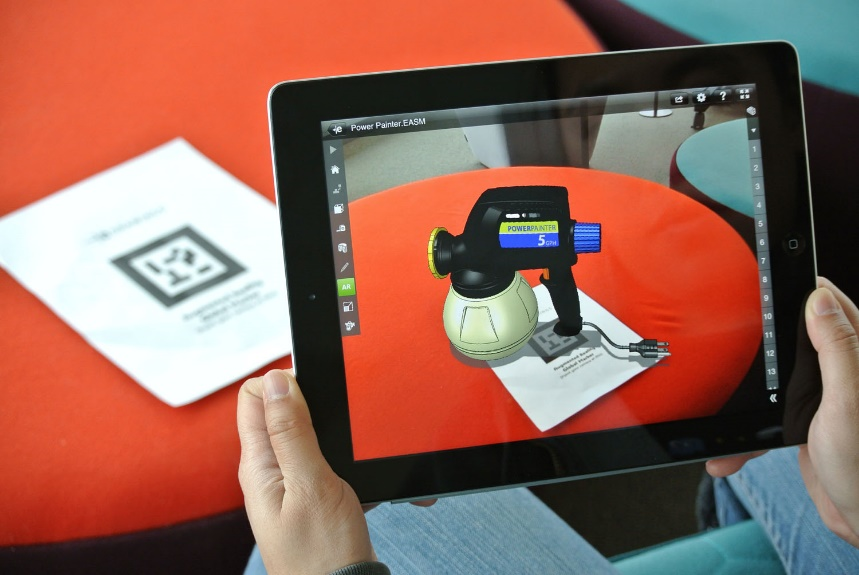
\includegraphics[width=240pt,height=180pt,keepaspectratio]{graphics/ARpad.png}
\caption{\cite{javaObjectClass}}
\end{figure}
[4]\\
\\
\subsection{Google Glasses}
The new innovation from google was really exciting. Google glass is a new gadget for the whole world. Furthermore it combines the reality with virtual components . This project’s launch event was in 2012 .Google Glass is the name for a type of wearable computer. It was created by the Google’s Project team Glass. It provides Augmented Reality for users by visually connecting them to an Android-run heads up display that offers many of the features of an Android smartphone. With this device the user can connect to Google’s key cloud features such as maps, calendar ,Gmail, Google+ and Google Places. Google hopes to have the gadget in the market in the near future. So they expect the technology to cost about as much as a smartphone. [5]
\\
\\
\begin{figure}[htbp]
\centering
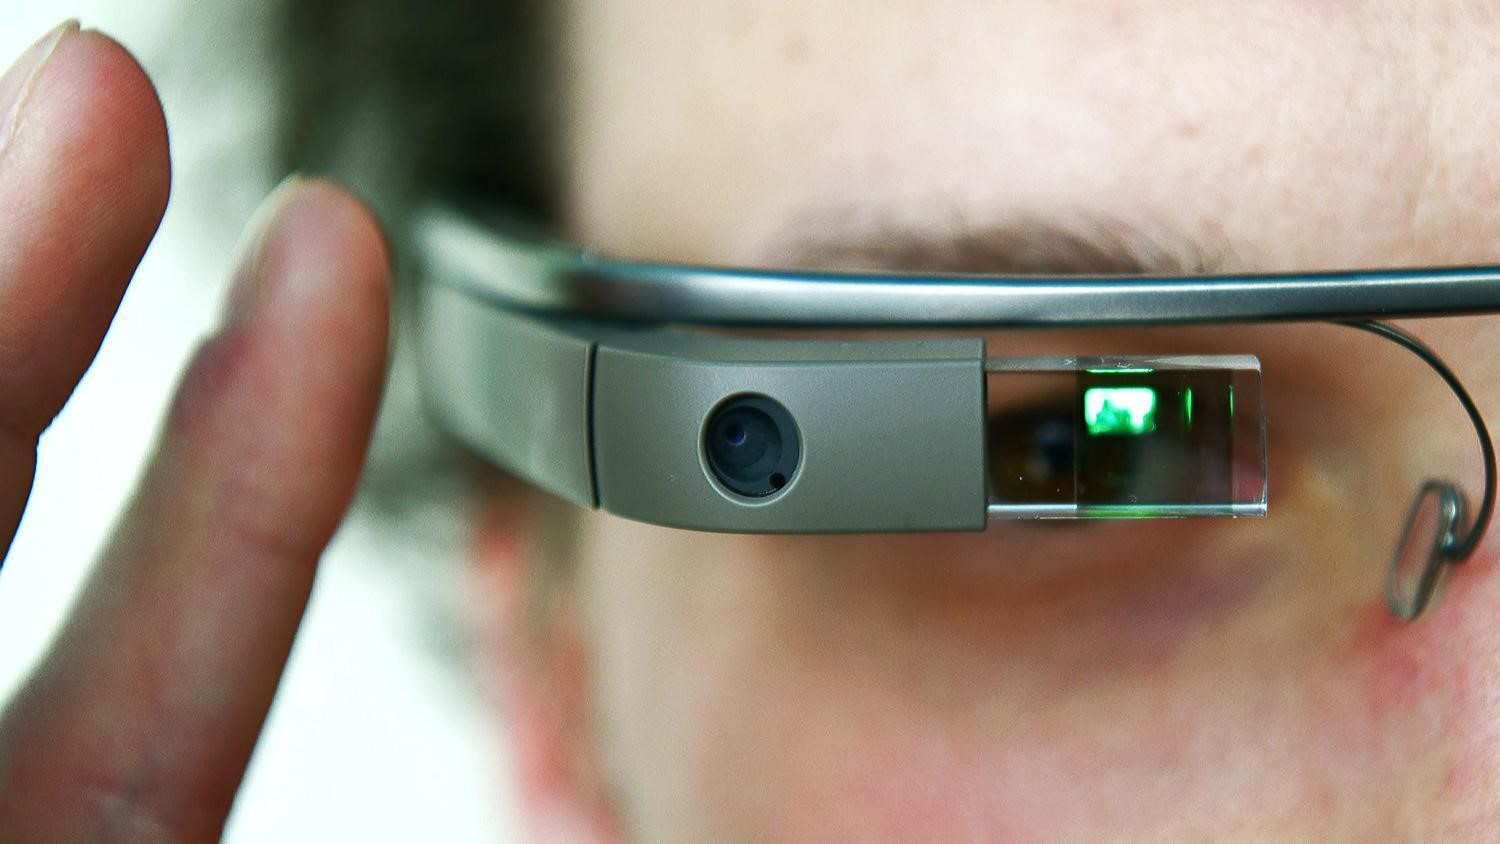
\includegraphics[width=240pt,height=180pt,keepaspectratio]{graphics/GoogleGlasses.jpg}
\caption{\cite{javaObjectClass}}
\end{figure}
\\
\\
Google Glass has 7 main functionalities[6]:
\\
\\
The first one ,it doesn’t need an extension of a smartphone or tablet. This gadget has it’s own hardware such as in mobile phones. It can perform itself various day to day tasks, without moving the hands of a user. 
\\
\\
The second function is that it can record a video or it will take picture, if the user just give an oral command. So in that case the user never have to touch a Button or the hardware. The photos and videos will be stored on the 4GB flash memory of the device and it can also be shared on social networking websites or emailed.
\\
\\
The third function is , it shows the user text messages as well as emails that the user receives. Via voice commands the user can reply to the text message or email.
\\
\\
The fourth function is about googling with this device. If the person like to find a lot of information , the user just have to ask a question and Google glass will pull the answer from the internet. For example ,the end-user can ask when the st. stephen's cathedral was built or to give a few pictures of the church. The answers or the pictures will be provide on the small screen in form of the users eye.
\\
\\
The next feature is to show maps. Probably lots of people uses Google Maps, so Google Maps are integrated into Glass. The user will be able to chart the course of the journey or lookup locations. It is possible to do establishments via voice commands.
\\
\\
The fifth feature is live video sharing. Google Glass has the ability to show the world what the user of the device sees $\rightarrow$ live! A good example is , when the user is attending a family function and users child’s school play or a concert, he/she can share the feed with her/his friends or family members in real-time. So he/she can make them a part of the experience.
\\
\\
Google Glass’s next features is , it has Google Now integrated. Google Now is a digital voice assistant. It will keep track of the daily habits , such as when the user leave for office of the route that the user take.  Google Now  will give the user a alternate routes if there is a traffic on the way or it gives weather updates periodically and it has among various other functions.
\\
\\
The last function from  Google Glass is, translation from a language to another. The user have to ask Google Glass to translate a phrase or sentence from one language to another and it will speak that out.
\\
\\
\begin{figure}[htbp]
\centering
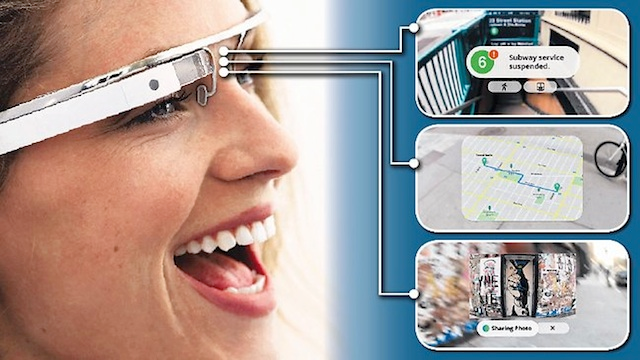
\includegraphics[width=240pt,height=180pt,keepaspectratio]{graphics/googlefunctions.png}
\caption{\cite{javaObjectClass}}
\end{figure}
[7]
\subsection{Usage of Augmented Reality[8]}
\subsubsection{Military and Law Enforcement }
The military and law enforcement agencies uses  AR Technology for  full simulators which are designed to help in training.  For Example, a wide screen inside a room or a vehicle on which various scenarios is presented, and the trainee must decide the best course of action.
\\
\\
Some advanced Special Forces teams have basic AR goggles that , along with the land in sight, display information such as altitude, angle of viewing, light intensity, and so on.AR technology also used by specialized night vision glasses. This device can display location and other information. The most of the unmanned vehicles in the military branches uses also AR technology as well. These vehicles, especially the aerial ones, can be thousands of kilometres away from their operators. The next point is that the vehicles have one or more cameras mounted on their exterior, which transmit video to their operator. This vehicle are equipped with several sensors as well. There is a sensor which sends data to the operator along with the video. This data is the processed and augmented over the video.  The operator’s System with complex algorithms picks out the mark building or objects of interest. This kind of information will be displayed as an overlay on the video.
\\
\\
\subsubsection{Vehicles}
Nowadays AR technology started to be implemented in vehicles. Often there are multiple screens in the vehicle, each showing particular direction. So just think about there is only one screen and multiple cameras, the vehicle will either switch the feed automatically or have the option for the user to switch  between the cameras. The exterior of the vehicle has the ability to control the several cameras. The images from the camera will be shown on the screen and it is overlayed with useful data such as small map, compass, direction arrows, alternate routes, weather forecast and much more. This kind of technology is currently most visible in airplanes and trains at the moment. Some smart cars has the same ability ,but they are in test phase . The Submarines and ships are using this technology as well. The important thing is that Space Shuttles had this kind of AR technology also.
\\
\\
It is possible to create apps which implement a sort of hybrid way on the Android platform. The reason is that the most Android devices seem to bee lacking in features that normal vehicles have, the same kind of features are not achieved. On the other hand, apps can be written for the help to navigate by using the GPS to get to the right location.  With the right API it is possible to write a APP to use the accelerometer to help with  acquiring the speed of the vehicle. Android device provides the AR power and the vehicle  provides the vehicle part.
\\
\\
A example of a smart car:
\begin{figure}[htbp]
\centering
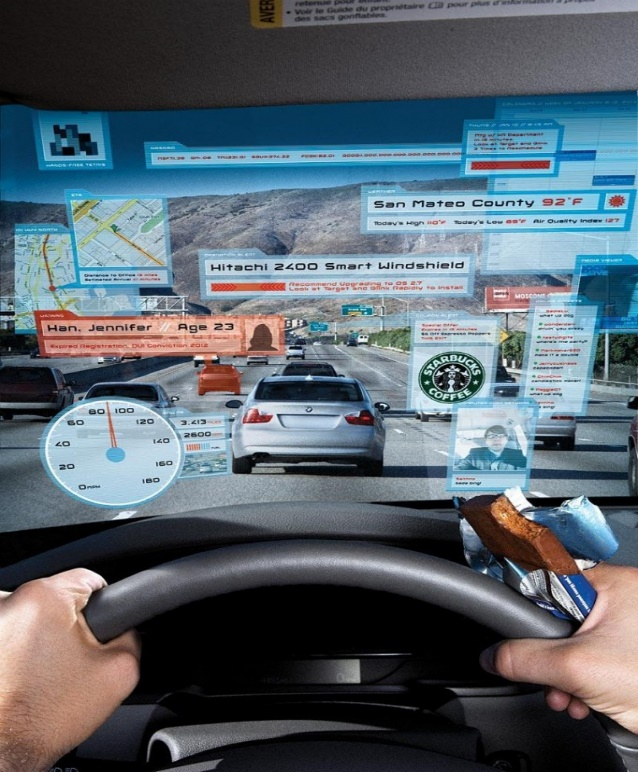
\includegraphics[width=240pt,height=180pt,keepaspectratio]{graphics/smartcar.png}
\caption{\cite{javaObjectClass}}
\end{figure}
[9]
\subsubsection{Medical}
AR technology is quite popular in the medical field.  This technology enables to becoming more common these days for surgeries.  With AR the error rate are smaller in Surgery branch. The reason is that the computer provides valuable inputs on the surgery and uses the information to control robots to perform some or all of the surgery.  Furthermore , the computer  can often provide alternative ways and instructions  on what can be done to improve the  surgery in real time.   Augmented Reality  stream , along with other data, these data can be sent per remote to doctors, who can view the information of the patient as  if the patient were in front of them.
\\
\\
In the medical field ,there are other medical apps of AR technology.  It is possible to use AR machines to monitor a large number of patients and make sure that their vital signs are under observation at all times.
\\
\\
This kind of AR technology can never be implemented on a Android smartphone. The main reason is , it is to expensive.  To create such a app we need a team of very good developers, a team of highly skilled and experienced doctors and a large amount of money.
\\
\\
\subsubsection{Trail Rooms}
AR technology are widespread in several shops. The reason is , why some shops uses AR is to create a virtual trial room.  The idea of virtual trial room is  that the user stands in front of a screen with a camera mounted somewhere.  So the user will see himself displayed on the screen. The next point is the user uses an input devices such as a mouse or a keyboard to select any of the available clothing options. In the background the computer use a algorithm to augment that item onto the user’s image and display it on the screen.  The  user can turn to view himself from all angles. 
\\
\\
\subsubsection{Tourism}
The Tourism branch is also using the AR technology.  Around the World, there are a lot of famous spots. So the organized tours now offer a head-mounted AR system that displays information about the current site and its buildings when the user look at it.  Furthermore the tourist can rebuild buildings, cities , landscapes and terrains as they existed in the past with the AR technology. The Tourism AR provide icons or markers for famous monuments. Tourism AR has the ability to find parks, restaurants, hotels and other tourist related sites and attractions in an unfamiliar city. These applications are not limited to historical places. 
\\
\\
\subsubsection{Architecture}
In this the world there a lot of camera-equipped machines that can generate a blueprint form an existing structure or display a virtual structure from the blueprints on the proceed site of constructions.  These functionality helps to design and check buildings. Augmented  reality technology provides the functionality to simulate natural disaster conditions. So it can show how the building structure will react under that kind of pressure.
\\
\\
\subsubsection{Education}
In Educational Institutes is AR technology very useful. Children or students can learn through AR. AR act in this field as  add-ons to the textbook material or as a virtual, 3d textbook in itself. Furthermore the AR give the ability for the student to “relive” events as they are known to have happened, while never leaving their class.
\\
\\
\subsubsection{Art}
Augmented Reality helps  to create paintings, models and other forms of art.  The technology helps  to try out a particular design, before  actually putting it down in ink or craving it out of stone. It is also able to paint something virtually to see how they turn out and the artist can repaint as often he wants until he is satisfied . Then he can put down on the canvas finally.
\\
\subsubsection{Translation}
AR technology can be used for translate text from multiple languages all over the world. AR feature OCR and either have an entire cross-language dictionary on the device or it can translate the language over the Internet.    Few companies are producing apps with this ability. For this function we have to use  a ready-made optical character recognition(OCR) library to convert the images from the camera to text. The idea of OCR is it extract the text from image and put compare it with the translation dictionary or it can be translated through the internet. The translated result will be shown on the display.
\\
\subsubsection{Weather Forecasting}
Most of the weather forecast app are augmented. The Data for the weather will be recorded and while the recording  the green backdrop serves as a  marker. If the recording is finished, a computer is used to add the map and position to match the forecaster’s actions. AR  are used by transmitting the forecast live to the viewers .
\\
\\
\subsection{Future of Augmented Reality[10]}
Augmented Reality is a growing up technology. It has amazing abilities, but few of the abilities can’t be implemented right now due to limitations in hardware and algorithms.
\subsubsection{Virtual Experiences}



In the future the AR technology could have a system ,which could transform from the current location into something completely different. A good example is , just imagine in the future you can live through movies by wearing  such a system and seeing the movie happen around. Probably this technology could convert the house of a user into a medieval castle or into the international space station. Furthermore with the combination  of smell-emitting technology and the aural AR , it could make the environment lifelike and  feel completely real. In addition to this ,it is capable to add a emulation of the sense of touch with a body suit. That will make it absolutely and undeniably real. 
\\
\\
\subsubsection{Holograms}
The following point is that AR allows  the user to have a live direct or indirect of the world. That could enable users to have holograms in front of them. These holograms could be interactive or merely descriptive.  For instance somebody is calling you and a hologram of these person appears in front of you. So we see AR could have this ability.
\subsubsection{Video Conferencing}
In the future , multiple people will appear in the same conference room if a video feed of a conference room is  transmitted to them with the AR technology.  The idea is that the people could use  the webcam to “appear” in the seat of the room, along with the members.
\\
\\
This idea could probably help people who are not able to attend the meeting ,because they are thousands of kilometres away. So this futuristic Video Conferencing could solve this problem. Furthermore for this implementation we need a high-speed internet and the person which participating the conference have to stay  exactly in the same place, if not then the algorithm have to positioning him again and these need a big amount of the data streaming.
\\
\\
\subsubsection{Movies}
This technology can be used  to play entire movies.  The idea is that the theatre could be replaced with the background of the movie  or the theatre could be replaced with the actors only.  The first method is that the actors could be augmented onto the background and in  other way the background could be augmented behind the actors. The second method would reduce the costs of the shooting. These methods could provide more realistic and fun movies.
\\
\\
\subsubsection{Gesture Control}
AR could be used for many gesture controls such as eye dialing.   It should track the eye movement from the user and should select the right the appropriate number key. If they key has been selected , the user could blink to press that number and then proceed to select the next key. This kind of algorithm could be implemented to control music players, mobile apps, computers and other form of technology.
\\
\\
To create app with this algorithm requires a few things:
\\
\\
First of all it needs a front camera with a reasonable resolution. The second thing is that the algorithm has to be well written to detect fine eye movements  and to convert it to the right information. This algorithm has to filter other movements.
\\
\\
\subsection{Summary}
So we see that AR is a developing technology. The basic requirements for the technology is back and front camera , GPS, accelerometer and compass. Most of the requirements are fulfilled by almost all Android devices on the market. Now is great time to create AR apps, because in these the competition is very low and it is good to start business with it. Augmented Reality are quite popular in many fields such as Military, Medical and Education.
\\
\\
\begin{figure}[htbp]
\centering
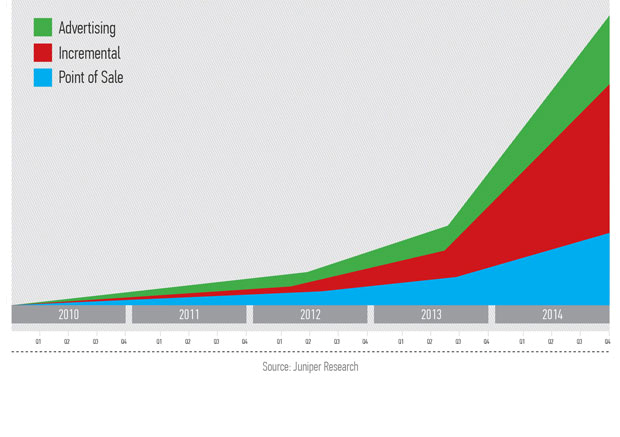
\includegraphics[width=240pt,height=180pt,keepaspectratio]{graphics/statistics.png}
\caption{\cite{javaObjectClass}}
\end{figure}
[11]
\\
The Graph is showing the Advertising and Point of Sale rate of AR. We can see the graph is increasing year to year. The Result of the Graph is that the features of the technology is increasing.

\section{Java}
\subsection{What is Java}
Java is a computing platform and object oriented programming language first released by Sun Microsystems in 1995. Oracle has bought Java in 2010.\cite{JavaWhat}
\\



The Java platform consists of the Java application programming interfaces (APIs) and the Java virtual machine (JVM).
\\



Java is class-bases and object oriented. It is intended to let application developers'write once, run anywhere' meaning that code that runs on one platform does not need to be recompiled to run on another. Java programs are compiled to byte-code. this code can run on any JVM regardless of the real computer architecture.\cite{javaWiki}
\\

Java is next to C/C++ one of the most popular programming languages.\cite{progLangPop} The language also has a similar syntax to C and C++.

\subsection{Class Based \& Object Oriented}
Class-based object-oriented languages, such as Java , are founded on the concept of two distinct entities: classes and instances.\cite{javaObjectClass} 

\begin{enumerate}
\item \textbf{Class:} A class is a blueprint or prototype from which objects are created. \cite{javaOBjectOracle} In class-based languages, you define a class in a separate class definition. In that definition you can specify special methods, called constructors, to create instances of the class. A constructor method can specify initial values for the instance's properties and perform other processing appropriate at creation time.\cite{javaObjectClass} In Java the \textbf{new} Operator is with a call of the constructor method is used to make a new instance of a class. 


\item \textbf{Instance:} An instance or object is the instantiation of a class that is one of its members. Software objects are often used to model the real-world objects

\item \textbf{Interface:} An interface is a collection of empty methods. When a class implements an interface, in java with the keyword \textbf{implements}, it has to implement all methods of the interface. A class describes the attributes and behaviors of an object. An interface contains behaviors that a class implements. 

\item \textbf{Subclasses:} In a class-based language, you create a hierarchy of classes through the class definitions.\cite{javaObjectClass} The subclass, in Java the keyword \textbf{extends} is used, provides all functionalities of the super class an can add new ones ore modify the existing properties.

\begin{figure}[htbp]
\centering
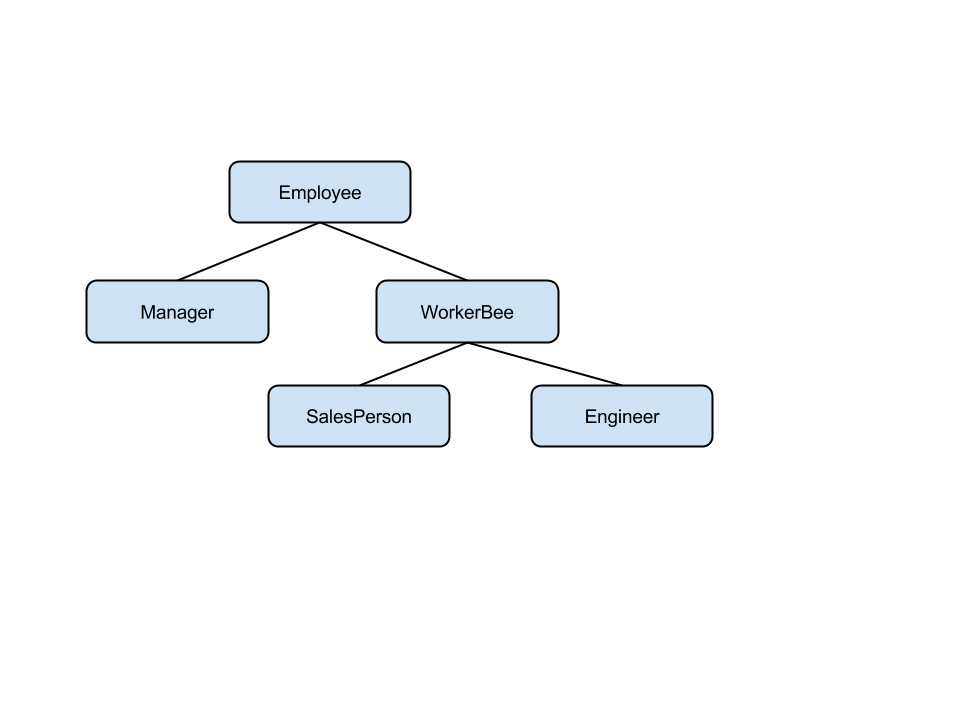
\includegraphics[width=240pt,height=180pt,keepaspectratio]{graphics/java_subclass.png}
\caption{\cite{javaObjectClass}}
\end{figure}
As you can see in this example \textit{Engineer} is an \textit{Employee}. But \textit{Manager} which also is an employee has not the same properties. 


\item \textbf{Abstract Class:}
An abstract class is a class that can't be instantiated. It's only purpose is for other classes to extend. Abstract classes are similar to Interfaces but an abstract class, in contrast, provides more structure. It usually defines some default implementations and provides some tools useful for a full implementation.\cite{javaAbstractVsInterface}

\item \textbf{Package:} 
A package is a namespace for organizing classes and interfaces. Packages make large software projects easier to manage. \cite{javaOBjectOracle}
\end{enumerate}


\subsection{Design Patterns}
Design patterns are proven solutions approaches to specific problems. A design pattern is not a framework! They are based on the base principles of object orientated design. 

\begin{enumerate}
\item Program to an interface not an implementation
\item Favor object composition over inheritance.
\end{enumerate}

\subsection{Performance}
Programs written in Java have the reputation of being slower than other languages. However in the last 10 years the JVM execution speed increased dramatically. In six separate web performance benchmarks, Java frameworks took 22 out of the 24 top-four positions. The JVM has been optimized that much that Java code is now running nearly as fast as C++ code. \cite{javaPerfromance}

\subsection{JVM}
The Java virtual machine is what makes Java a platform independent programming language. A virtual machine (VM) is a software implementation of a machine (i.e. a computer) that executes programs like a physical machine. Therefore, the JVM runs on all kinds of hardware to execute the Java Bytecode without changing the Java execution code. Java developers do not need to know how the JVM exactly works. However a deeper knowledge of the JVM helps understanding how JAVA works and can be helpful to solve various problems.\cite{javaJVM} 
\\


Features of JVM:
\begin{enumerate}
\item \textbf{Stack-based virtual machine:} Most computer architectures such as Intel x86 Architecture and ARM Architecture are based on registers. Whereas the JVM is stack based.\cite{javaJVM} That means that the VM doest need to know the operand addresses, it only calls the Stack-Pointer which points to the current instruction. \cite{stackBased_vs_registerBased} 
\item \textbf{Symbolic reference:} All data types except for primitives are referred to through a symbolic reference.   
\item \textbf{Garbage collection:} The garbage collector frees the memory from objects that are not in use any more. \cite{javaGarbageCollector}  
\item \textbf{Guarantees platform independence by clearly defining the primitive data type:} In other more tradition languages like C or C++ primitive data types have different sizes according to the System. In Java the JVM defines a fixed size for primitives. 
\end{enumerate} \cite{javaJVM}

\subsection{Java bytecode}
The Java bytecode is the result of a compiled Java source-code. It is a middle-language between Java and the machine code. \cite{javaJVM}  

\subsection{Java Code Execution Process} 
The Java code execution process is shown in the following figure. 
\begin{figure}[htbp]
\centering
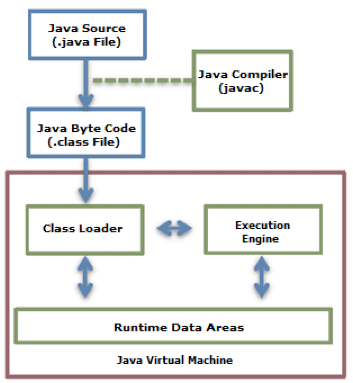
\includegraphics[width=\textwidth,height=\textheight,keepaspectratio]{graphics/java-code-execution-process.png}
\caption{java code execution process \cite{javaJVM}}
\end{figure}
\subsubsection{Class Loader}
The Java Class Loader loads and links a class when it refers to a class the first time at runtime. Every class loader has its own namespace that stores the loaded classes.\cite{javaJVM} 

\subsubsection{Runtime Data Areas}
The JVM Runtime Data Areas is the Memory assigned to a program when it runs on the OS. They can be divided into six areas: the Pc Register, JVM Stack, Native Method Stack, Heap, Method Area, and the Runtime Constant Pool. The first three are created for a single thread the other areas are shared by all threads.  

\begin{enumerate}
\item \textbf{PC register:} One \textbf{program counter} register exists for one thread. It gets created when the thread starts. Pc register has the address of the JVM instruction that is executed now.\cite{javaJVM}
 
\item \textbf{JVM Stack:} Each thread has a private JVM Stack, created the same time as the thread. A Java Virtual Machine stack stores frames. Frames are used to store data and results, new frames are created each time a method is invoked. It gets destroyed when its method invocation completes, whether that completion is normal or abrupt (it throws an uncaught exception). \cite{javaVMOracle}

\item \textbf{Native Method Stack:}
A stack for native code written in a other language than Java. It is a stack used to execute C od C++ Methods.\cite{javaJVM}.  

\item \textbf{Heap:}
The JVM Heap is a data area that is shared among all Java Threads. The heap is created on virtual machine start up.
Its a space that stores all class instances Arrays and Variables. If a program requires more heap space than aviable the Java Virtual Machine throws an \textbf{OutOfMemoryError}\cite{javaVMOracle}

\item. \textbf{Method area:} The method area is shared by all threads, created when the JVM starts. It stores runtime constant pool, field and method information, static variable, and method bytecode for each of the classes and interfaces read by the JVM. Unlike in the heap the garbage collection in the method area is optional for each JVM version. \cite{javaJVM}

\item \textbf{Runtime constant pool:}
The Runtime pool is a part of the Native Method stack and gets created when a class or interface gets created. Its the run-time representation of the \textbf{constant pool} table in a class file. This constant pool table contains several constants \cite{javaVMPaper}

For example:
\begin{lstlisting}[language=Java, caption=Java example Code]
System.out.println("Hello, world!");
\end{lstlisting}
Generated byte-code:
\begin{lstlisting}[language=Java, caption= JVM bytecode]
0:   getstatic       #2;               
3:   ldc     #3;                         
5:   invokevirtual   #4; 
\end{lstlisting}
\#n indicates that this is a reference to the constant pool.
2 is a symbolic reference to \textit{System.out}, \#3 is the \textit{Hello, world!} string.\#4 references to the \textit{PrintStream.println(String)} method.
\cite{javaVmstover}  
\end{enumerate}
\begin{figure}[htbp]
\centering
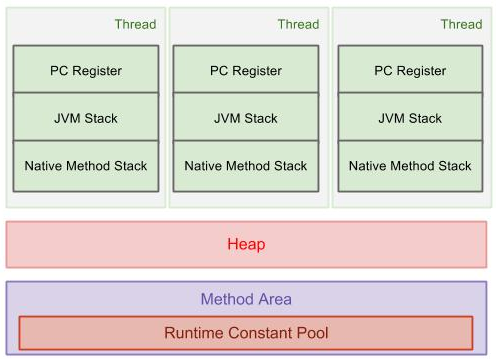
\includegraphics[width=\textwidth,height=\textheight,keepaspectratio]{graphics/java-data-areas.png}
\caption{Java Run-time Data Areas \cite{javaDataAreas}}
\end{figure}
\newpage

\subsubsection{Execution Engine}
The bytecode that is assigned to the runtime data areas in the JVM loaded from the class loader is executed by the execution engine. The execution engine reads the Java Bytecode in the unit of instructions. It is like a real CPU executing the machine commands one by one. Each command consists of 1 Operation Code byte and an additional Operand code. The execution engine gets one OpCode and execute task with the Operand, and then executes the next OpCode.\cite{javaJVM}  

\subsection{.JAR File}
A JAR \textbf{(Java ARchive)}is a file  that contains the class, image, sound, etc. files for a Java application or applet gathered into a single file and possibly compressed. \cite{javaJarMargaret}

\subsubsection{Executable JAR }
Its also possible to create a executable .Jar files. It behaves similar to a .exe file in Windows. It can be executed with a double click when Java is installed on the system. 


%%%%%%%%%%%%%%%%%%%%%%%%%%%%%%%%%%%%%%%%%
\chapter{Typographic Design}
\label{ch:typo}
%%%%%%%%%%%%%%%%%%%%%%%%%%%%%%%%%%%%%%%%%


For working with LaTeX you can take advantage of a variety of books and free introductions and tutorials on the internet. A competent contact point for LaTeX beginners is the LaTeX Wikibook, which is available under \url{http://en.wikibooks.org/wiki/LaTeX}. 

The following sections give examples of the most important LaTeX environments and commands.

\section{Tables}
\subsection{Tableeee}
Tables have to be realized with the help of the \textit{table} environment. Tables shall be sequentially numbered for each chapter and described in terms of a short caption (cf. Table~\ref{tab:diplomaseminar}).

\begin{table}[htb]
	\centering
	\begin{tabular}{|l|c|c|}
		\hline \textbf{Name} & \textbf{Date} & \textbf{Title} \\
		\hline
		\hline Mustermann Adam  & 18.5   & T1    \\
		\hline Musterfrau Eva  & 22.6   & T2    \\
		\hline
	\end{tabular}
	\caption{Seminar for Master Students}
	\label{tab:diplomaseminar}
\end{table}


\section{Figures}

Like tables, figures shall be sequentially numbered for each chapter and described in terms of a short caption). You could either produce your drawings directly inside Latex using PSTricks\footnote{\url{http://tug.org/PSTricks}}, Tikz\footnote{\url{http://sourceforge.net/projects/pgf}}, or any set of macros dedicated to your requirements (cf. Figure~\ref{fig:samplefigure_tikz}). Alternatively, you may include figures prepared in external tools (cf. Figure~\ref{fig:samplefigure_pdf}). Note, to ensure high quality printing, all figures must have at least 300 dpi.

\begin{figure}
	\centering
	\begin{tikzpicture}[->, auto, node distance=2.8cm, semithick]
	  \node[initial, state] (1)		 {$S_1$};
	  \node[state] 		(2) [right of=1] {$S_2$};
	
	  \path (1) edge [bend left]  node {0} (2)
		(1) edge [loop above] node {1} (1)
		(2) edge [bend left]  node {0} (1)
		(2) edge [loop above] node {1} (2);
	\end{tikzpicture}
	\caption{Sample figure}
	\label{fig:samplefigure_tikz}
\end{figure}

\begin{figure}[tb]
	\centering
	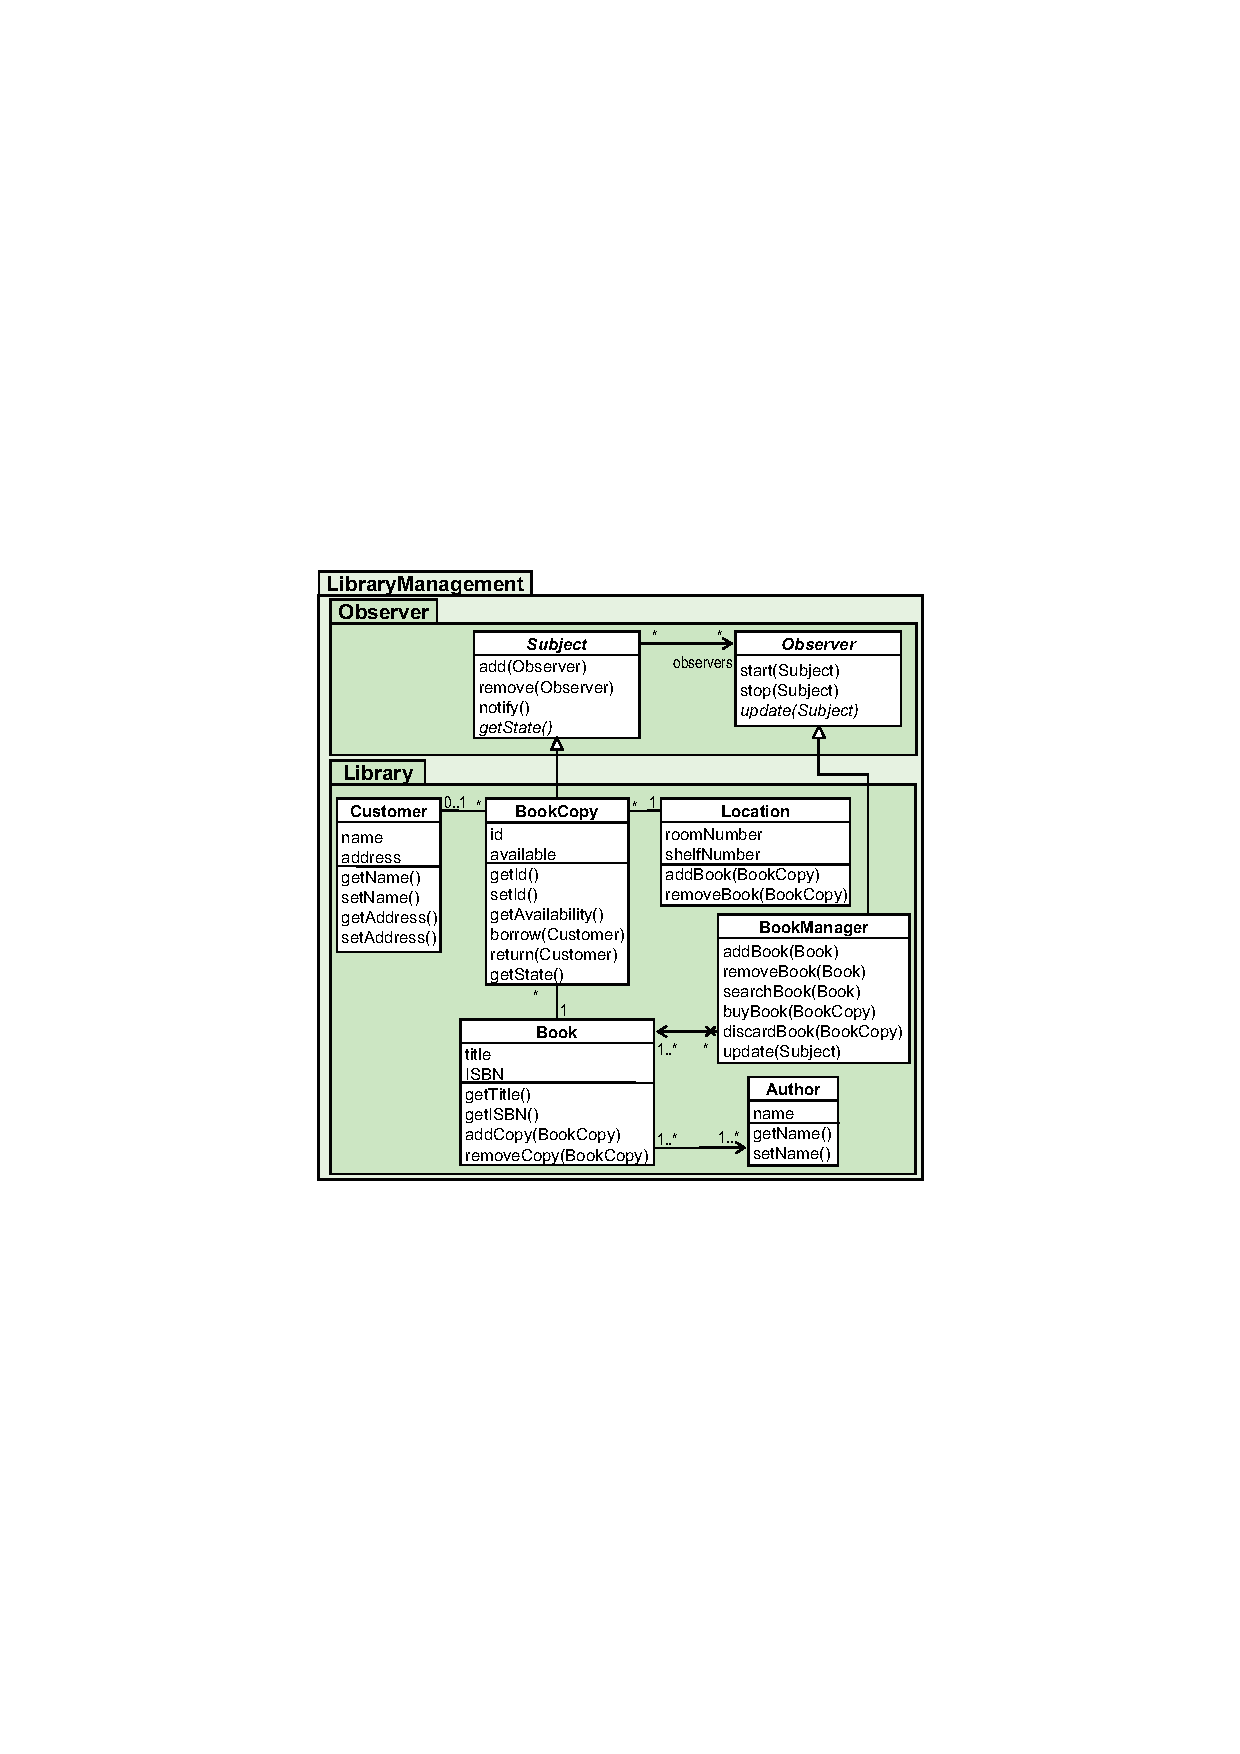
\includegraphics[width=0.7\textwidth]{figures/figure1}
	\caption{Sample figure}
	\label{fig:samplefigure_pdf}
\end{figure}


\section{Fonts}

When introducing important terms for the first time use \emph{emphasize}. For a consistent look and feel of proper names like {\cd} and {\uml{Observer}} pattern you may define macros in the main document \texttt{thesis.tex}.

\section{Code}

For short code fragments use the \textit{verbatim} environment.

\begin{verbatim}
//Start Program
System.out.println("Hello World!");
//End Program
\end{verbatim}

A much better alternative is the \textit{algorithm} environment (cf. Algorithm~\ref{alg:samplealgorithm}). This environment offers special formatting features for loops, operations and comments.

\begin{algorithm}[t]
\SetKwData{Left}{left}
\SetKwData{This}{this}
\SetKwData{Up}{up}
\SetKwFunction{Union}{Union}
\SetKwFunction{FindCompress}{FindCompress}
\SetKwInOut{Input}{input}
\SetKwInOut{Output}{output}

\Input{A bitmap $Im$ of size $w\times l$}
\Output{A partition of the bitmap}

\BlankLine

\emph{special treatment of the first line}\;
\For{$i\leftarrow 2$ \KwTo $l$}{
\emph{special treatment of the first element of line $i$}\;
\For{$j\leftarrow 2$ \KwTo $w$}{\label{forins}
\Left$\leftarrow$ \FindCompress{$Im[i,j-1]$}\;
\Up$\leftarrow$ \FindCompress{$Im[i-1,]$}\;
\This$\leftarrow$ \FindCompress{$Im[i,j]$}\;
\If(\tcp*[r]{O(\Left,\This)==1}){\Left compatible with \This}{\label{lt}
\lIf{\Left $<$ \This}{\Union{\Left,\This}}\;
\lElse{\Union{\This,\Left}\;}
}
\If(\tcp*[r]{O(\Up,\This)==1}){\Up compatible with \This}{\label{ut}
\lIf{\Up $<$ \This}{\Union{\Up,\This}}\;
\tcp{\This is put under \Up to keep tree as flat as possible}\label{cmt}
\lElse{\Union{\This,\Up}}\tcp*[r]{\This linked to \Up}\label{lelse}
}
}
\lForEach{element $e$ of the line $i$}{\FindCompress{p}}
}
\caption{Sample algorithm}\label{alg:samplealgorithm}
\end{algorithm}



\chapter{Integrated Development Environment}


%George, Pokorny
\section{Andorid SDK Eclipse}




















%Korabach
\section{JetBrains WebStorm}
The application’s logic had to be created with a programming language called JavaScript. Because of that, the project group had to find a development environment that’s best suited for this language. JetBrains WebStorm 7.0.3 was best fit for all future tasks and should be the environment in which JavaScript had been developed. 
\\

However, not only JavaScript, but also HTML as well as CSS could be developed with this IDE. All information about this product can be found on Jet Brains homepage.\cite{webstorm}
\subsection{Overview}
JetBrains WebStorm is a professional JavaScript IDE that supports a wide range of modern technologies related to JavaScript programming language, HTML and  CSS, and provides the complete experience for productive Web development.
\\

WebStorm offers developers an intelligent code editor that truly supports the structure of code written in JavaScript, HTML or CSS, as well as their modern  successors. It features the best-of-breed coding assistance for a whole set of  cutting-edge web technologies, including code completion, refactorings, code formatting, on-the-fly error prevention, and much more. 
\\

WebStorm is also great for developing Node.js applications. Together with integrated instruments 
for testing, debugging and code analysis and integration with various VCS, WebStorm is an essential tool for powerful and productive web development.
\\

\begin{figure}[h]
\centering
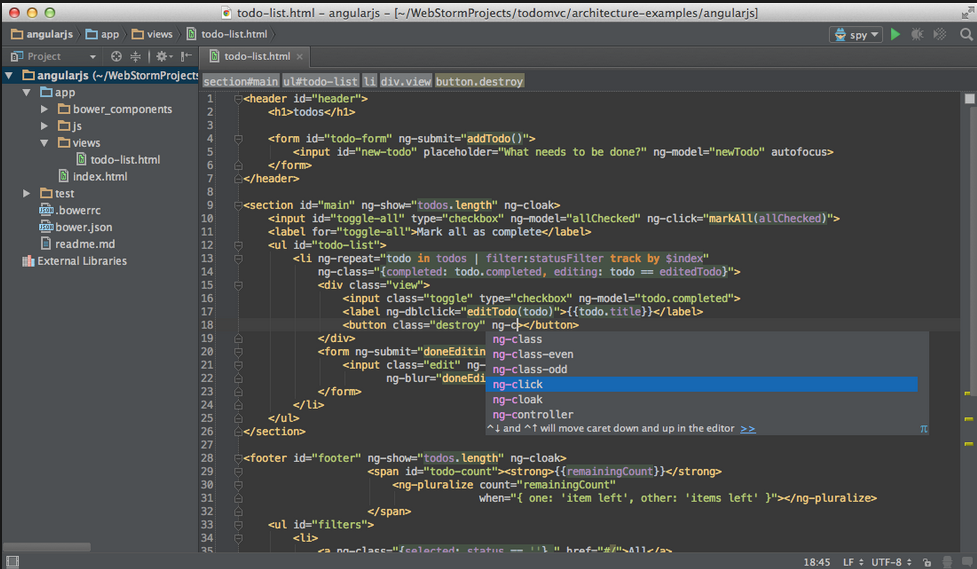
\includegraphics[width=1\linewidth]{graphics/chapter3/1}
\caption{WebStorm Interface}
\label{}
\end{figure}


\subsection{Features}
\begin{itemize}
\item Intelligent JavaScript, HTML, and CSS editor with syntax highlighting, code completion, configurable formatting configuration, refactorings, on-the-fly error detection and support of language mixtures.
\item Support for a wide range of technologies: TypeScript, CoffeeScript, Dart, LESS, Sass, Stylus, Compass, EJS, Handlebars, Mustache, Web Components, Jade, Emmet, and many more.
\item Productivity-boosting Live Edit feature: See the changes in the browser immediately without reloading the page.
\item 
JavaScript debugger for Chrome and Firefox, with breakpoints, stepping, frames view and watchers. Full-featured debugging of TypeScript, CoffeeScript and Dart with sourcemaps.
\item 
File Watchers for automatic compilation/transpilation of higher-level languages like TypeScript, CoffeeScript, LESS, Sass, and Stylus.
\item 
A debugger for Node.js applications with the latest features of V8 Debugger Protocol.
\item 
Intelligent code inspections, one-click quick-fix suggestions, JSHint, JSLint, and Google Closure Linter.
\item
JavaScript unit testing with integrated JSTestDriver or Karma test runner with code coverage. 
\item
Built-in HTTP Server, REST Client, Terminal and Node.js package manager npm. 
\item 
New Project Wizard with well-known project templates like Twitter Bootstrap and Node.js Express App.
\item
Integration with Version Control Systems including Git, Subversion, Mercurial, CVS, Perforce, and GitHub. 
\item 
Easily configurable FTP/FTPS/SFTP deployment.
\item 
Integration with various issue trackers.
\end{itemize}
















%Fegerl
\section{Visual Studio}


% % % % % % % % % % % % % % % % % % % % % %
\chapter{Implementation in JavaScript} \label{chapter:desgin}

The logic of this app is divided into two parts. First part is JavaScript logic, that is responsible for the functionalities of each HTML site, more precisely, the dynamic response to the user. Second part is Java Android logic, which is responsible for the main function called car tracking and all other functionalities that could not be accomplished with help of JS. 
\\

Altogether there are 10 HTML sites and each one of them has some functionalities that had to be implemented with JS or Android Java. A simple example of a functionality is pressing a button. This button triggers a function inside the JS. 
\\

However, JavaScript and Android Java did not provide everything that has been needed for the project application. That's the reason why project members had to use several other web frameworks like jQuery or phonegap.js. This was necessary to accomplish the main goal of a powerful, user-friendly mobile application. The usage of web frameworks will be explained in following chapters. 
\newpage



\section{Display}
This chapter describes the functionality behind each display of mobile application. 


\subsection{Start Menu}
The Start menu is displayed after the application was started. It provides user with several functions like help, car tracking, favourite list, about and exit. Basically it is the first thing that user sees and from there he navigates threw the whole application.
\\

\begin{figure}[h]
\centering
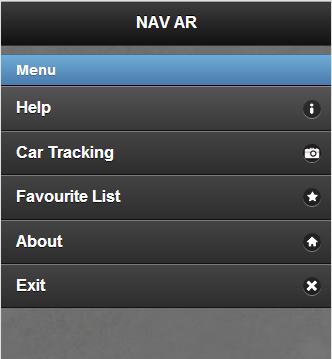
\includegraphics[width=0.5\linewidth]{graphics/chapter4/1}
\caption{Start menu}
\end{figure}


Each one of these buttons have their logic that is implemented in \textbf{index.html}.
\newpage The listing 4.1 shows the functionality behind each button.
\\

\begin{lstlisting}[language=html, caption= 
Start menu source code,captionpos=b]
<li data-icon="info">
  <a href="help.html" rel="external">
    Help
  </a>
</li>
<li data-icon="camera">
  <a href="#" onclick="trackClick();">
    Car Tracking
  </a>
</li>
<li data-icon="star">
  <a href="myfavourite.html" rel="external">
    Favourite List
  </a>
</li>
<li data-icon="home">
  <a href="about.html" rel="external">
    About
  </a>
</li>
<li data-icon="delete">
  <a href="#" onclick="turnOff();">
    Exit
  </a>
</li>
\end{lstlisting}


\
\
Functions \textit{trackClick()} and \textit{turnOff()} were implemented in Android Java and are described in chapter 5)''Implementation in Android Java and Metaio Tracking''.
\\


\begin{lstlisting}[language=html, caption= 
JavaScript functions in start menu,captionpos=b]
function trackClick() {
    MyTracking.performClick();
}

function turnOff(){
	Exit.exitClick();
}
\end{lstlisting}


The button \textbf{help} forwards the user to the help display \textit{help.html}. The same functionality features \textbf{about} and \textbf{favourite list}, except they link to another display. 
\\

\textbf{Exit} button invokes the function \textit{turnOff()} which calls another Android Java implemented function. \textit{Exit.exitClick()} ends the application. Illustrated in listing 4.2.
\\

\textbf{Car tracking} calls a function \textit{trackClick()}. This method starts the main function.
\\
\newpage


\subsection{Help}
The help display provides only two major options: back button and the link to a tutorial video. This tutorial was created by the project members and is an YouTube video.


\begin{figure}[h]
\centering
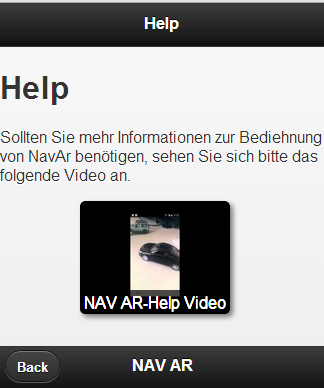
\includegraphics[width=0.5\linewidth]{graphics/chapter4/2}
\caption{Help display}
\end{figure}


The back button leads to the main menu. Shown in listing 4.3.
\\
\begin{lstlisting}[language=html, caption= 
Back button,captionpos=b]
<a class="ui-btn-left" href="index.html" rel="external">
	Back
</a>
\end{lstlisting}
\
\


If the user touches the picture \textbf{NAV AR - Help Video}, he will be linked to a specific how-to YouTube video. This video serves as a simple help to understand how the application works. It shows how to use the application's main functions and more.
\\

\begin{lstlisting}[language=html, caption= 
Help video,captionpos=b]
<a href="https://www.youtube.com/watch?v=6U4oT5AbAsre">
  NAV AR-Help Video
</a>
\end{lstlisting}


%%%%%%%%%%%%%%%%%%%%%%%%%%%%%%%%%%%%%%%%%%%%%%%%%%%%%%%%%%%%%%%%%%
%New Chapter Main Menu
%%%%%%%%%%%%%%%%%%%%%%%%%%%%%%%%%%%%%%%%%%%%%%%%%%%%%%%%%%%%%%%%%
\subsection{Main Menu}
The most important function of the whole mobile applications is \textbf{car tracking}. This function is executed by \textit{MyTracking.peformClick()}. More in chapter 4.1)''Start Menu''.
\\

After a car was successfully tracked, the user is linked to a new display called \textbf{index.html}, which is the start menu. It provides the user with additional options. Options that deliver technical information as well as review about the tracked car and more other useful functions. 
\\

There is also a possibly to add the tracked car to users car collection named \textbf{the favourite list}. Out of there he can select one specific vehicle to use the start menu options, like picture or videos gallery.
\\

JavaScript functions had to be created for each  of this options. These functions are described in chapter 4.3.1)''JavaScript Functions''.
\\

\begin{figure}[h]
\centering
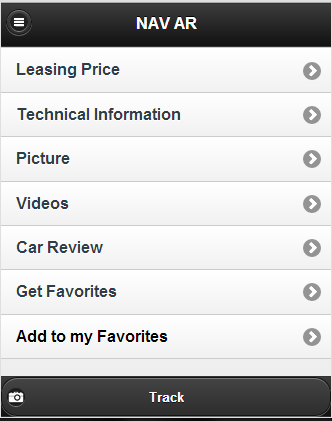
\includegraphics[width=0.5\linewidth]{graphics/chapter4/3}
\caption{Main Menu}
\end{figure}
\newpage


\
Listing 4.23 shows the function behind each button. Some buttons only link to another, other invoke specific functions like \textit{LocalStorageWriteId()}.\\
\begin{lstlisting}[language=html, caption= 
Main menu source code,captionpos=b]	
<li>
  <a href="leasingprice.html" rel="external">
    Leasing Price
  </a>
</li>
<li>
  <a href="technicalinfo.html" rel="external">
    Technical Information
  </a>
</li>
<li>
  <a href="slide.html" rel="external">
    Picture
  </a>
</li>
<li>
  <a href="video.html" rel="external">
    Videos
  </a>
</li>
<li>
  <a href="#" rel="#" onclick="reviewClick();">
    Car Review
  </a>
</li>
<li>
  <a href="myfavourite.html"rel="external">
    Get Favorites
  </a>
</li>
<li>
  <a id="add_favorite" 
  onclick="LocalStorageWriteId
  (sessionStorage.getItem('id'),globalcarname);"
   style="color:red" rel="external">
     Add to my Favorites
  </a>
</li>
\end{lstlisting}
\newpage


\subsubsection{Leasing Price}
%%%%%%%%%%%%%%%%%%%%%%%%%%%%%%%%%%%%%%%%%%%%%%%%%%%%%%%%%%%%%%%%%%%%
%link to chapter with leasing price technologie
%%%%%%%%%%%%%%%%%%%%%%%%%%%%%%%%%%%%%%%%%%%%%%%%%%%%%%%%%%%%%%%%%%%%
When the user presses on button \textbf{leasing price} he will be linked to the html page \textit{leasingprice.html} where he receives informations about the specific vehicle. \\
\
\

\begin{figure}[h]
\centering
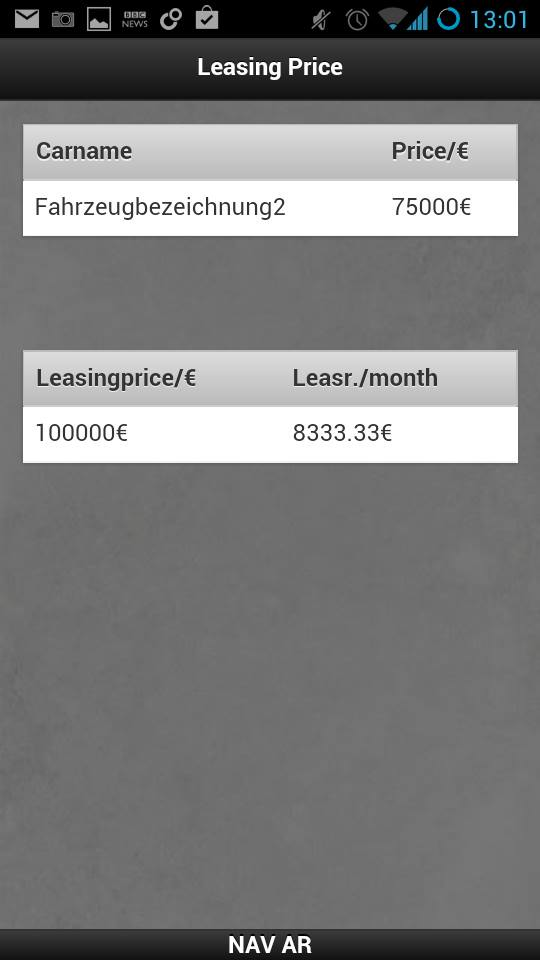
\includegraphics[width=0.5\linewidth]{graphics/chapter4/5}
\caption{Leasing Price}
\end{figure}
\newpage


\subsubsection{Technical Information}
By calling \textbf{technical information} facts about a specific car are presented. To create it several new features had to be used. Phone Gallary and Dynamic Selection of Colour. Informations about those are featured in chapters 4.6)''Photo Gallery'' and  4.8)''Dynamic Selection of Colours''.
\\

\begin{figure}[h]
\centering
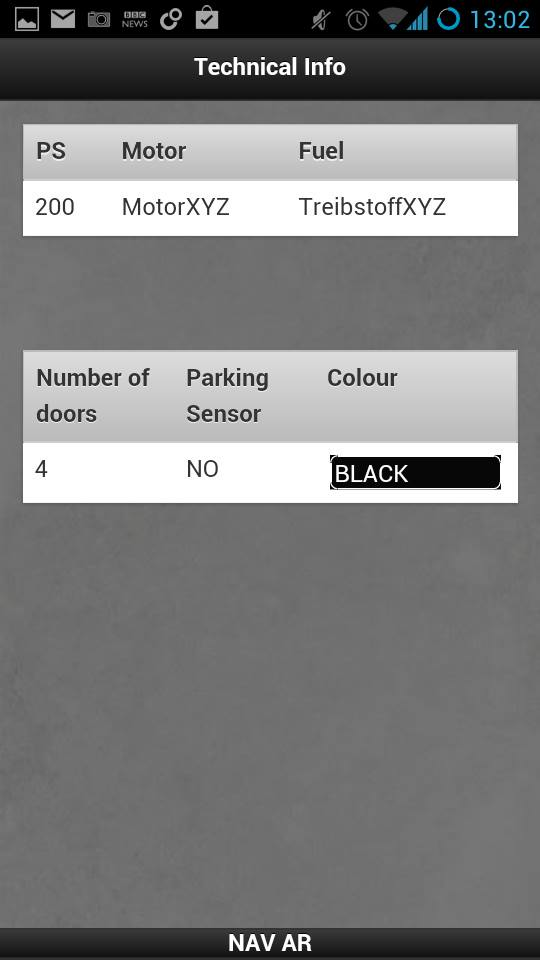
\includegraphics[width=0.5\linewidth]{graphics/chapter4/6}
\caption{Technical Information}
\end{figure}
\newpage

\subsubsection{Pictures}
Has freshest pictures of the specific car. Feature called Photo Gallery in chapter ..... was used to create this option.

\begin{figure}[h]
\centering
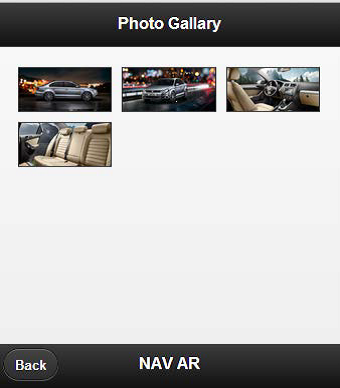
\includegraphics[width=0.5\linewidth]{graphics/chapter4/7}
\caption{Pictures}
\end{figure}
\newpage

\subsubsection{Videos}
This option provides the user with videos about the selected car from favourite list or fresh tracked one. More about video gallery in chapter.....
\\
\begin{figure}[h]
\centering
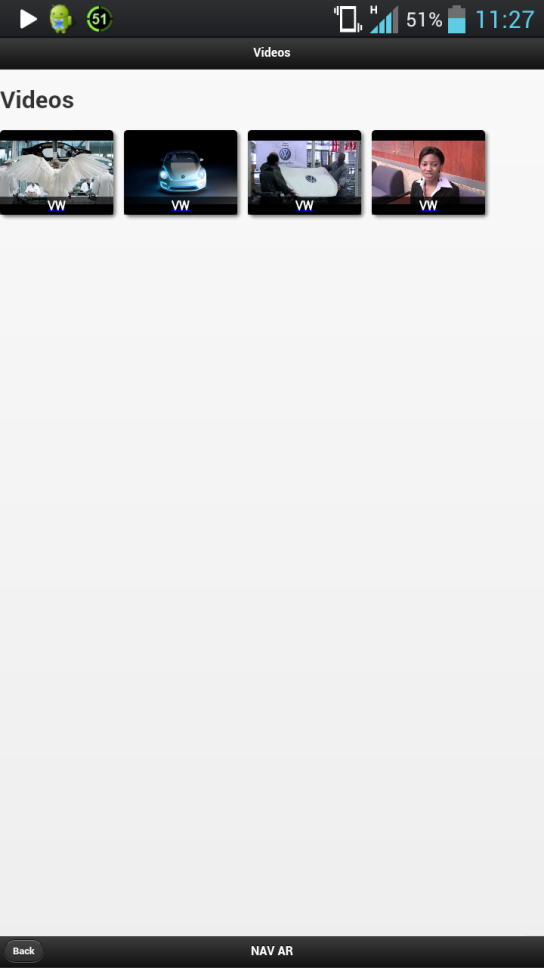
\includegraphics[width=0.5\linewidth]{graphics/chapter4/8}
\caption{Video Gallery}
\end{figure}
\newpage

\subsubsection{Review}
Operation review invokes a self created method called \textit{reviewClick()}. Description to thisit is in chapter 4.3.1 Created Methods, Review. Basically review links the user to a new display where he can read review about the specific car.
\\

\begin{figure}[h]
\centering
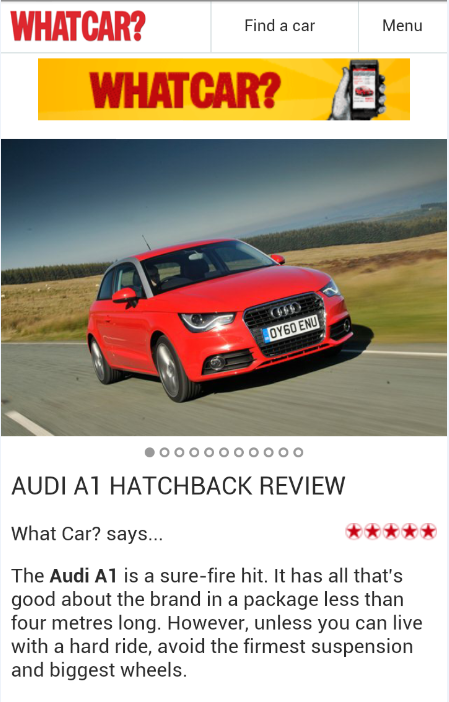
\includegraphics[width=0.5\linewidth]{graphics/chapter4/9}
\caption{Review}
\end{figure}
\newpage


\subsubsection{Get Favourites}
This operations links the user to his favourite cars which he saved with the option \textbf{add to my favourite}. Information about the favourite list in chapter 4.4)My Favourites.
\\

\begin{figure}[h]
\centering
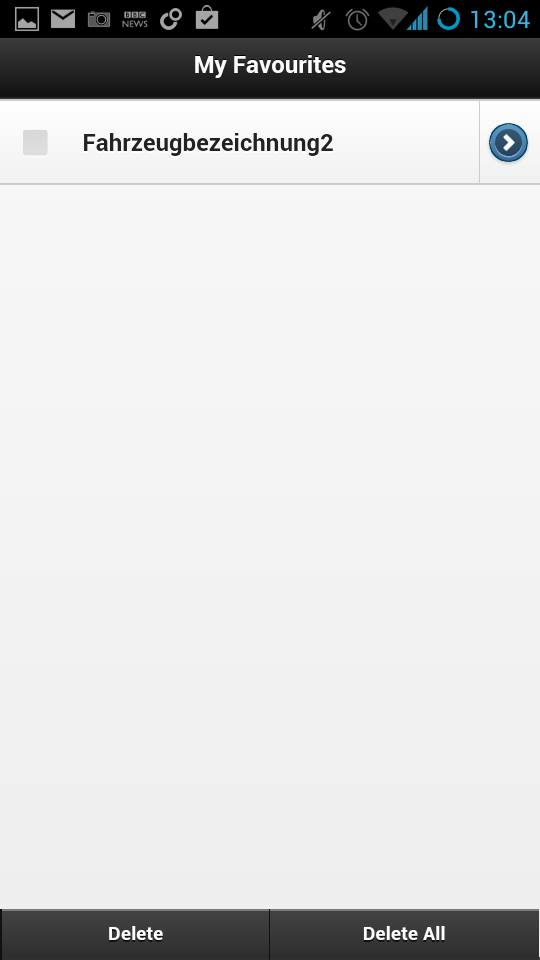
\includegraphics[width=0.5\linewidth]{graphics/chapter4/10}
\caption{Favourite list}
\end{figure}
\newpage

\subsubsection{Add to my Favourites}
The button \textbf{Add to my Favourites} trigger the function \textit{LocalStorageWriteId()}. It saves the id and the name of the tracked car into users favourites. For the first parameter it takes the tracked car id from the session storage. For the second parameter the global variable \textit{globalcarname}.
\\

\begin{lstlisting}[language=html, caption= 
add favourite sorce code,captionpos=b]
<li>
  <a id="add_favorite"onclick="LocalStorageWriteId
  (sessionStorage.getItem('id'),globalcarname);"
  style="color:red" rel="external">
    Add to my Favorites
   </a>
</li>
\end{lstlisting}
\

\
Before the user can add the vehicle to his favourites he has to wait several seconds. In this time the request is send to the server for information about the car threw its id. If the user wants to access the operation in its loading time, the application denies him the access and informs him about the loading time.
\\

\begin{figure}[h]
\centering

\includegraphics[width=0.65\linewidth]{graphics/chapter4/11}
\caption{Not ready function}
\end{figure}
\

The operations colour changes from red to black when the function is loaded.
\\
\begin{figure}[h]
\centering

\includegraphics[width=0.65\linewidth]{graphics/chapter4/12}
\caption{Ready function}
\end{figure}
\newpage

\subsection{My Favourites}
Inside the favourites are cars had been added threw the operation \textbf{add to my favourites}. The favourite cars can be selected or deleted. Removing the cars from favourites is possible by selecting the specific vehicle or removing all of the cars.
\\

\begin{figure}[h]
\centering
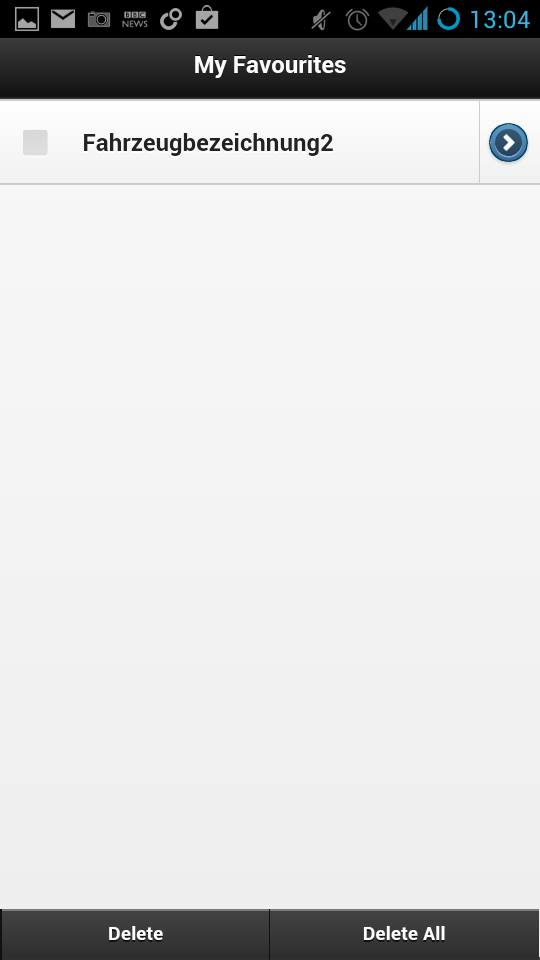
\includegraphics[width=0.4\linewidth]{graphics/chapter4/15}
\caption{My Favourites display}
\end{figure}
\



\subsubsection{Loading of favourite cars}
Before the functions of the favourite list can be used, the list entries(cars) have to be initialized. This is done automatically when the site is loaded. 
\\

Each line that is written inside document.ready starts after the document is ready. This is where the favourite cars are initialized.
\\
\newline
\newline

\begin{lstlisting}[language=html, caption= 
source for document is ready,captionpos=b]
$(document).ready(function () {
.
});
\end{lstlisting}
\

First, all car names are loaded from local storage into an array called \textit{storedCarNames}. So this array is filled with vehicle names which user added to his favourites. 
\\

\begin{lstlisting}[language=html, caption= 
Array with favourite cars,captionpos=b]
var storedCarNames = JSON.parse(localStorage["fcarname"]); 
\end{lstlisting}
\


Now the filling of the cars into a list begins. The loop goes so long as the number of cars in the array. In this loop a car name is put into the \textit{listItem1} which is just a panel shown in figure 4.17.
\\

Next \textit{listItem1} is put into another list. This list is where all panels(favourite cars) are stored. Each new vehicle is put into the list.
\\
\begin{lstlisting}[language=html, caption= 
Adding list items into the list,captionpos=b]
for (var i = 0; i < storedCarNames.length; i++){
  var key = storedCarNames[i];
  listItem1 = '"specific list item"';

  $('#liste').append(listItem1);
}
\end{lstlisting}

\begin{figure}[h]
\centering

\includegraphics[width=0.7\linewidth]{graphics/chapter4/16}
\caption{A list item}
\end{figure}

Last but not least the list that has to be refreshed so the list items are displayed. 
\\

\begin{lstlisting}[language=html, caption= 
Refreshing the list,captionpos=b]
$('#liste').listview('refresh').trigger('create'); 
\end{lstlisting}


\subsection{About}
The \textbf{about} display has no logic and no self made functions except one the back button which functionality you have learnt in 4.2)Help chapter.
\\
\begin{figure}[h]
\centering
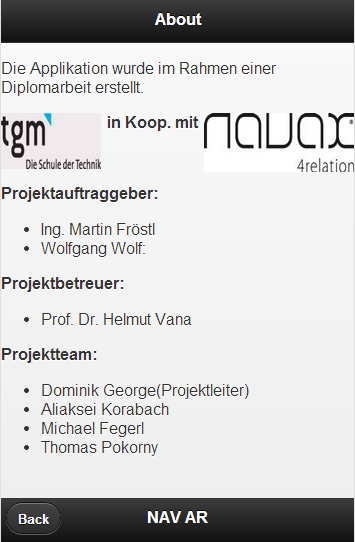
\includegraphics[width=0.4\linewidth]{graphics/chapter4/17}
\caption{About display}
\end{figure}
\newpage


\section{Implemented Function}


\subsection{Start timer}
When the site is loaded a timer automatically starts. Specific functions stop the timer and sends the time stamp to the NAV server.
\\
\begin{lstlisting}[language=html, caption= 
Start timer function,captionpos=b]
function startTime(){
	var d = new Date();
	timestart = d.getTime();
}
\end{lstlisting}

\subsection{End timer}
This function stops the timer which had been started with the method \textit{startTime()} and safes the time with the method \textit{timestampsave()}. The timer was used to get the time how long a user has selected a specific car and used certain start menu options.
\\

\begin{lstlisting}[language=html, caption= 
End timer function,captionpos=b]
function endtime(){
	var d = new Date();
	var endtime = d.getTime();
	timestampsave(timestart,endtime);
}
\end{lstlisting}


\subsection{Save the time}
This function saves start time and end time of the timer, into the NAV server. The start time and end time are the input parameters. 
\\

%%%%%%%%%%%%%%%%%%%%%%%%%%%%%%%%%%%%%%%%%%%%%%%%%%%%%%%%%%%%%%%%%%
%link to michaels chapter about the connection
%%%%%%%%%%%%%%%%%%%%%%%%%%%%%%%%%%%%%%%%%%%%%%%%%%%%%%%%%%%%%%%%%%

To save the time into the server \textit{timestampsave()} needs several other information like email and id of the tracked car. More about sending information to the server and  to the connectivity between application and server read the chapter 7.0.3.4)''Communication from mobile device to the C App''.
\\

time1.....start time
\\
time2.....end time\\
\newline


\begin{lstlisting}[language=html, caption= 
Save time function,captionpos=b]
function timestampsave(time1,time2){
  var stime	= time1;
  var endtime = time2;
  var emailan = sessionStorage.getItem('email');
  var fid = sessionStorage.getItem('id');
    
  $(document).ready(function () {
     $.ajax({
        type: "GET",
        url: "URL",
        async: false,
        dataType: 'JSONP',
        success: function(data){
        //do your stuff with the JSON data
          var test=data;
          console.log(test);
        }
     });
  });
}
\end{lstlisting}


\subsection{Set parameters}
There are two parameters that have to be saved into the session storage to establish a connection with the NAV server. That were id of the tracked car and the email address of the user.
\\
\begin{lstlisting}[language=html, caption= 
Set parameter function,captionpos=b]
function setParam(){
	window.sessionStorage.setItem('id', myVariable);
	window.sessionStorage.setItem('email',email);
}
\end{lstlisting}

%%%%%%%%%%%%%%%%%%%%%%%%%%%%%%%%%%%%%%%%%%%%%%%%%%%%%%%%%%%%%%%%%%
%link to chapter with car tracking in java android
%%%%%%%%%%%%%%%%%%%%%%%%%%%%%%%%%%%%%%%%%%%%%%%%%%%%%%%%%%%%%%%%%%
\subsection{Start car tracking}
This function starts to track a car. For more explanation refer to chapter 5)'Implementation in Android Java and Metaio Tracking'.
\\
\newline
\newline
\begin{lstlisting}[language=html, caption= 
Car tracking function,captionpos=b]
function trackClick() {
  MyTracking.performClick();
}
\end{lstlisting}

%%%%%%%%%%%%%%%%%%%%%%%%%%%%%%%%%%%%%%%%%%%%%%%%%%%%%%%%%%%%%%%%%
%link to chapter with the revie in android java
%%%%%%%%%%%%%%%%%%%%%%%%%%%%%%%%%%%%%%%%%%%%%%%%%%%%%%%%%%%%%%%%%
\subsection{Review}
This method is implemented with Java Android. More about in chapter 5)'Implementation in Android Java and Metaio Tracking'.
\\

\begin{lstlisting}[language=html, caption= 
Review function,captionpos=b]
function reviewClick(){
        Review.performClick();
    }
\end{lstlisting}

%%%%%%%%%%%%%%%%%%%%%%%%%%%%%%%%%%%%%%%%%%%%%%%%%%%%%%%%%%%%%%%%%
%link to chapter java android implementation
%%%%%%%%%%%%%%%%%%%%%%%%%%%%%%%%%%%%%%%%%%%%%%%%%%%%%%%%%%%%%%%%%
\subsection{Turn off}
This function is implemented with Android Java and has been documented in 4.1)''Start Menu''.
\\

\begin{lstlisting}[language=html, caption= 
Turn off funtion,captionpos=b]
function turnOff(){
        Exit.performClick();
    }
\end{lstlisting}


\subsection{Home}
This function returns the user back to the start menu and is implemented with Android Java.\\

\begin{lstlisting}[language=html, caption= 
Home function,captionpos=b]
function home(){
        Home.performClick();
    }
\end{lstlisting}


\subsection{Read car name}
This method returns the name of the car that had been tracked threw a car specific id. Each transport has its own unique id. This id is predefined and set after the tracking was successful. Later it is stored in session storage.
\\
\newline  
%%%%%%%%%%%%%%%%%%%%%%%%%%%%%%%%%%%%%%%%%%%%%%%%%%%%%%%%%%%%%%%%%%
%link to chapter with ajax
%%%%%%%%%%%%%%%%%%%%%%%%%%%%%%%%%%%%%%%%%%%%%%%%%%%%%%%%%%%%%%%%%%
So the input parameter \textit{cname} is that specific id of the tracked or selected car. The name of the car is stored in the NAV server. A request had to be send to receive the name. More about Connectivity in chapter 7)''Streaming''.
\\

%%%%%%%%%%%%%%%%%%%%%%%%%%%%%%%%%%%%%%%%%%%%%%%%%%%%%%%%%%%%%%%%%%
%set code on one line
%%%%%%%%%%%%%%%%%%%%%%%%%%%%%%%%%%%%%%%%%%%%%%%%%%%%%%%%%%%%%%%%%%

\begin{lstlisting}[language=html, caption= 
Read car name function,captionpos=b]
function readcarname(cname){
  var test = '';
  $(document).ready(function () {
    $.ajax({
      type: "GET",
        url:"URL",
        async: false,
        dataType: 'JSONP',
        success: function(data){
          test=data.split(';');
          globalcarname=test[0];
          document.getElementById("add_favorite").
          style.color="black";
        }
    });
  });
}
\end{lstlisting}

%%%%%%%%%%%%%%%%%%%%%%%%%%%%%%%%%%%%%%%%%%%%%%%%%%%%%%%%%%%%%%%%%%
%link to chapter with ajax
%%%%%%%%%%%%%%%%%%%%%%%%%%%%%%%%%%%%%%%%%%%%%%%%%%%%%%%%%%%%%%%%%%
\subsection{Save email}
As the name says, \textit{saveEmail()} saves the email of a user. The information about users email was already stored in session storage through the function \textit{setParam()}. More in chapter 5.4)''Get Email Account from an Android device''.\\

Later this email is send to the NAV server. More about connection between app and server in chapter 7)''Streaming''.
\\

\begin{lstlisting}[language=html, caption= 
Save email function,captionpos=b]
function saveEmail(){    
  var value3 = sessionStorage.getItem('email');
  $(document).ready(function () {
     $.ajax({
     type: "GET",
     url: "URL",
       async: false,
       dataType: 'JSONP',
       success: function(data){
       //do your stuff with the JSON data
         var test=data;
         console.log(test);
       }
     });
  });
}
\end{lstlisting}

\subsection{Save car}
This function saves the id and the name of the tracked vehicle. This method is used for adding new cars to users car collection. In this function a feature called local storage that provides HTML5 for its users, was used. The function can be split into four phases.
\\

Phase one checks if the input parameter \textit{name} is not empty. If it is empty user receives information about it, otherwise it processes with the other phases.

\begin{lstlisting}[language=html, caption= 
Phase one,captionpos=b]
if(name!=null){
.....
}else{
  alert("Function is loading.");
}
\end{lstlisting}
\
\
\newpage
Phase two is the search phase. It searches for unique local storage place threw specific name \textit{(favorites ,fcarna)} and inspects if the storage with the name exists. If it doesn't exists an empty array is put inside the two local storages, else nothing happens.
\\

\begin{lstlisting}[language=html, caption= 
Phase two,captionpos=b]
if ((localStorage.getItem("favorites") === null) &&
 (localStorage.getItem("fcarname") == null)) {
   var names = [];
   localStorage["favorites"] = JSON.stringify(names);	
   localStorage["fcarname"] = JSON.stringify(names);
}
\end{lstlisting}


In phase three variables \textit{storedIds} and \textit{storedNames} are filled with information inside the local storage \textit{favorites} and \textit{fcarname}.
\\

\begin{lstlisting}[language=html, caption= 
Phase three,captionpos=b]
var storedIds = JSON.parse(localStorage["favorites"]);
var storedNames = JSON.parse(localStorage["fcarname"]);
\end{lstlisting}

Phase four checks if the car exists in the local storage. If it does the user receives information that this car already exists in the favourite list, else the id and car name is saved into the local storage.
\\

\begin{lstlisting}[language=html, caption= 
Phase four,captionpos=b]
if(storedIds.indexOf(id)>-1){
  Notifier.error('Car already exists.');
}else{
  storedIds.push(id);
  storedNames.push(name);
  localStorage["favorites"] = JSON.stringify(storedIds);
  localStorage["fcarname"] = JSON.stringify(storedNames);
  Notifier.success('Car has been added.');
}
\end{lstlisting}

The listing 4.19 shows the hole function with its four phases.\\
\begin{lstlisting}[language=html, caption= 
Save car function,captionpos=b]
function LocalStorageWriteId(id,name){
 if(name!=null){
  if((localStorage.getItem("favorites")===null)&&
   (localStorage.getItem("fcarname")==null)){
	var names = [];
	localStorage["favorites"] = JSON.stringify(names);
	localStorage["fcarname"] = JSON.stringify(names);
  }		
  var storedIds = JSON.parse(localStorage["favorites"]);
  var storedNames = JSON.parse(localStorage["fcarname"]);	
  if(storedIds.indexOf(id)>-1){
   Notifier.error('Car already exists.');
  }else{
   storedIds.push(id);
   storedNames.push(name);
   localStorage["favorites"] = JSON.stringify(storedIds);
   localStorage["fcarname"] = JSON.stringify(storedNames);
   Notifier.success('Car has been added.');
  }
  }else{
   alert("Function is loading.");
  }
}
\end{lstlisting}



\subsection{Delete favourite car}
This method deletes selected car with help of check box. If no car is selected, nothing happens by clicking on the button.
\\

\begin{lstlisting}[language=html, caption= 
Delete function,captionpos=b]
function deleteF(){
  Array.prototype.clean = function(deleteValue) {
   for (var i = 0; i < this.length; i++) {
       if (this[i] == deleteValue) {         
        this.splice(i, 1);
	    i--;
	   }
    }
    return this;
  };
	
var storedNames = JSON.parse(localStorage["favorites"]); 
var storedCarNames = JSON.parse(localStorage["fcarname"]); 
var lengthof=0;

for(var s=0;s<storedNames.length;s++){
  if(document.getElementById(s).checked){
    delete storedNames[s];
    delete storedCarNames[s];
	lengthof++;
  }		
}
if(lengthof!=0){
  Notifier.success('Cars deleted.');
  storedNames.clean(undefined);
  storedCarNames.clean(undefined);
  localStorage["favorites"]=JSON.stringify(storedNames);
  localStorage["fcarname"]=JSON.stringify(storedCarNames);
}
 window.location.reload();
}
\end{lstlisting}

\subsection{Delete all favourite cars}
Removes all favourite cars without selecting them.

\begin{lstlisting}[language=html, caption= 
Delete all function,captionpos=b]
function deleteAll(){
    Notifier.success('All cars have been deleted.');
	localStorage.clear();
    window.location.reload();
}
\end{lstlisting}

\subsection{Select favourite car}
Each car inside the favourite list can be selected. After the car is selected, the user is linked to the start menu.
\\

\begin{lstlisting}[language=html, caption=
Select car function,captionpos=b] 
function EventHandler(){
  Notifier.success('Car is selected.');
  var id = this.id;
  var storedNames = JSON.parse(localStorage["favorites"]);
	
  for(var i=0; i<storedNames.length;i++){
   if(id==i){
    window.sessionStorage.setItem('id', storedNames[i]);
   }
  }
}
\end{lstlisting}






















\section{Features}
Several new technologies were used to create the start menu. This chapter describes all those technologies. Some are linked to other chapters where they have already been explained. 
\\


\subsection{Local Storage}

HTML5 provides us with a new feature called Web Storage. In other words, with it web pages can store data locally within the user's browser or mobile application.
\\

Earlier, this was done with cookies. However, Web Storage is more secure and faster. The data is not included with every server request, but used ONLY when asked for. It is also possible to store large amounts of data, without affecting the website's performance.\cite{w3school}
\\

The data is stored in name/value pairs, and a web page can only access data stored by itself. Unlike cookies, the storage limit is far larger (at least 5MB) and information is never transferred to the server.\cite{w3school}
\\

HTML5 Web Storage provides two new objects for storing data on the client:
\begin{enumerate}
\item window.localStorage - stores data with no expiration date\cite{w3school}
\item code.sessionStorage - stores data for one session (data is lost when the tab is closed)\cite{w3school}
\end{enumerate}


\begin{figure}[h]
\centering
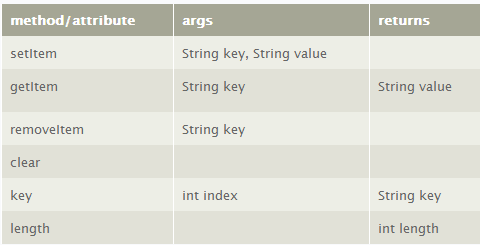
\includegraphics[width=0.9\linewidth]{graphics/chapter4/20}
\caption{Methods and attributes of local storage\cite{localstorageapi}}
\end{figure}


Here is an example of \textit{setItem} and \textit{getItem} in local storage.
\\

\begin{lstlisting}[language=html, caption= 
setItem example (Adapted from \cite{localstorageexample}),captionpos=b]
var foo = localStorage.getItem("bar");
// ...
localStorage.setItem("bar", foo);
\end{lstlisting}

In these application not a string but an array is stored inside the local storage. Here is an example how we put an empty array into a local storage.
\\

\begin{lstlisting}[language=html, caption= 
array into local storage,captionpos=b]
var names = [];
localStorage["favorites"] = JSON.stringify(names);
\end{lstlisting}
\
\

Here an example how we received the array form local storage.
\\
\begin{lstlisting}[language=html, caption= 
start timer function,captionpos=b]
var storedIds = JSON.parse(localStorage["favorites"]);
\end{lstlisting}

\newpage


\subsection{Slide Panel}
%%%%%%%%%%%%%%%%%%%%%%%%%%%%%%%%%%%%%%%%%%%%%%%%%%%%%%%%%%%%%%%%%%%%%
%link to slide panel chapter
%%%%%%%%%%%%%%%%%%%%%%%%%%%%%%%%%%%%%%%%%%%%%%%%%%%%%%%%%%%%%%%%%%%%%
In the upper left corner of the display exists a small button that calls the slide panel to open. More about slide panel in chapter 6.1.0.4)Slide Panel.
\\

\begin{figure}[h]
\centering
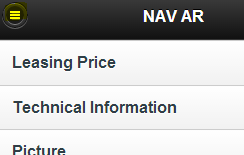
\includegraphics[width=0.5\linewidth]{graphics/chapter4/13}
\caption{Slide panel}
\end{figure}

After opening the slide panel more options are available. 
\\

\begin{figure}[h]
\centering
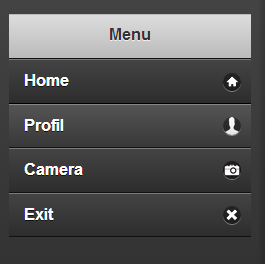
\includegraphics[width=0.5\linewidth]{graphics/chapter4/14}
\caption{Options of slide panel}
\end{figure}
\newpage

Here has the user four new options. He can return to the start menu with the display \textbf{home} or he can accesses his profile with \textbf{profil}. Also he can start to track a new car with \textbf{camera}. If the user doesn't want use the mobile application any more, he can close it the button \textbf{exit}. 
\\
\begin{lstlisting}[language=html, caption=Source code of slide panel options,captionpos=b]
<ul data-role="listview" data-theme="a">
  <li data-icon="home" >
    <a href="#" onclick="endtime();home();">
      Home
    </a>
  </li>
  <li data-icon="profil">
    <a href="profile.html" rel="external">
      Profil
    </a>
  </li>
  <li data-icon="camera" >
    <a href="#" onclick="endtime();trackClick();">
      Camera
    </a>
  </li>
  <li data-icon="delete">
    <a href="#" onclick="endtime();turnOff();">
      Exit
    </a>
  </li>
</ul>
\end{lstlisting}

The \textbf{home} button not only returns the user to the start menu but also ends the timer that has been started after a car was tracked. In addition, this timer is send straight to the NAV server.  
\\

Display \textbf{profil} calls to another display, in which the user can see his profile data. 
\textbf{Camera} function ends the timer and starts the tracking function. Exit ends the application.
\newpage


\subsection{Photo Gallery}
In this subchapter it describes the functionality of the photo gallery . The photo gallery is a feature of this project NAVAR. This feature shows the picture of the car which has been tracked by the NAVAR App. The Photo gallery is a plugin  from the photo swipe webpage. The Logic of the Photo swipe is implemented in a javaScript Library from photo swipe$\rightarrow$ klass.min.js. The functionality of the Design is defined in a css file$\rightarrow$ photoswipe.css. In this project it combined the Library form the photo swipe with the Library from jQuery Mobile. Furthermore the Table shows a Code snippet how to use the Library for this project:
\begin{figure}[h]
\centering
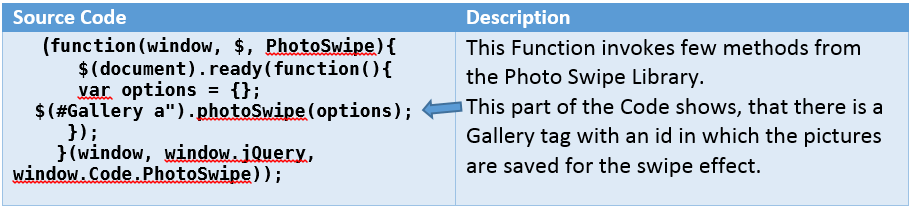
\includegraphics[width=1.0\linewidth]{graphics/photoswipe.PNG}
\caption{Photoswipe}
\end{figure}

Furthermore the pictures are saved on a server and in the Gallery we saved the URL of these pictures. The URL's are saved in an Array which has the id Gallery. For each car there is an Array with URL's of the pictures. Besides the photo swipe has the function to set a automatic Diashow.\\\\

\subsection{Sessionstorage}
Moreover the function called Sessionstorage is one of the big functionalities in this project. The Sessionstorage saves the value not persist, it means if the App is closed or has been ended  the value will be persistant . In the next Session or if the App has been started , there will be a new Sessionstorage. In this case the Project NAVAR uses the Sessionstorage to save the ID from the car, which has been tracked. Sessionstorage allows  to save a large amount of  key/value pairs and lots of text. This feature is impossible to do  via cookie. This kind of functionality uses  a protocol to save the Data. This protocol checks if the key and the value are a string, but if not it convert them to a string. Furthermore if a key was already present, its entry  has to be removed and the new one will be appended. The SessionStorage has it own methods for specific functionality.\\\\

First method is used to tell how many key/pair the SessionStorage contains. This method has the same function ,which tells the length of an Array, HTMLCollection \dots

\begin{figure}[h]
\centering
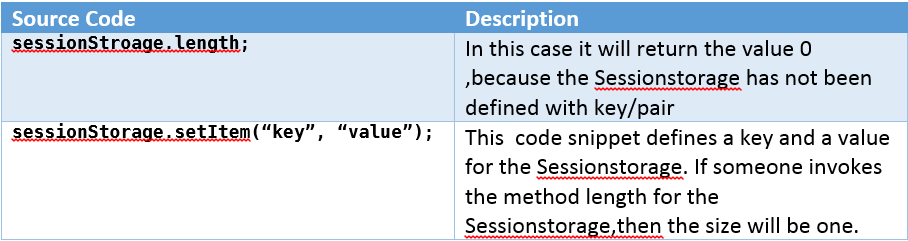
\includegraphics[width=1.0\linewidth]{graphics/sessionstorage1.PNG}
\caption{Sessionstorage}
\end{figure}

The second Method of Sessionstorage is called \textit{setItem(key:string,data:string)}.
 This method stores  a specified key  and the data. But if the key has been already stored and it uses the same key it will be overwritten. $\rightarrow$Example for setItem:\textbf{ sessionStorage.setItem('testkey','testvalue')}.
The third function is to get Data from the a specified key ,which has been already set. This method accepts any sort of string ,which has been used as key and returns the associated string as value or null if the key has not been stored before. Example:\\

\begin{figure}[h]
\centering
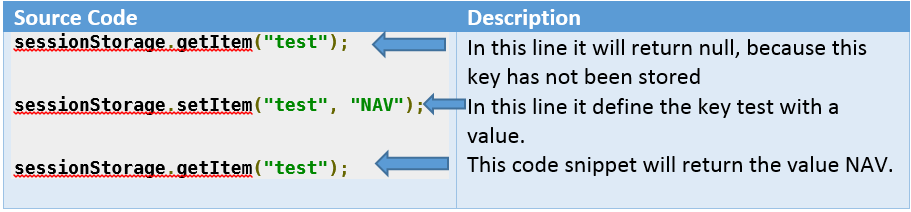
\includegraphics[width=1.0\linewidth]{graphics/sessionstorage2.PNG}
\caption{Sessionstorage}
\end{figure}

The last function is how to remove the key if it has no need for the Session. Example:
\begin{figure}[h]
\centering
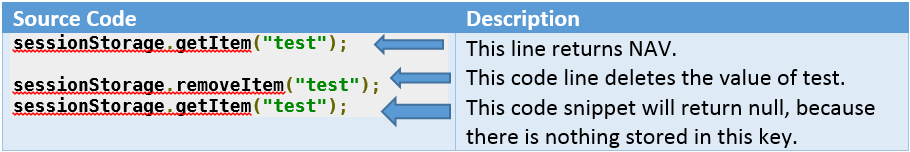
\includegraphics[width=1.0\linewidth]{graphics/sessionstorage3.PNG}
\caption{Sessionstorage}
\end{figure}

\subsection{Dynamic Selection of Colour}
This product has the feature to select the colour of the car . In the Technical Information the user has the opportunity to chose the colour of the Car, which has been tracked. The following code in the Figure shows how to create a dynamic selector with JavaScript:

\begin{figure}[h]
\centering
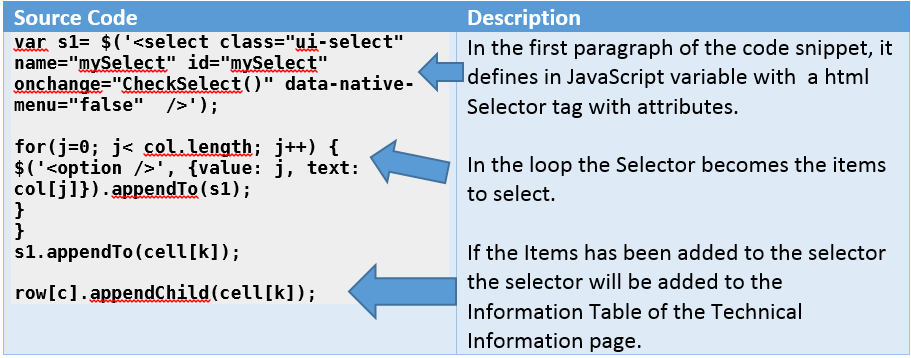
\includegraphics[width=1.0\linewidth]{graphics/Sessionstorage41.PNG}
\caption{Selector descritpion}
\end{figure}

\clearpage
The following picture shows how the Technical Info table looks like:

\begin{figure}[h]
\centering
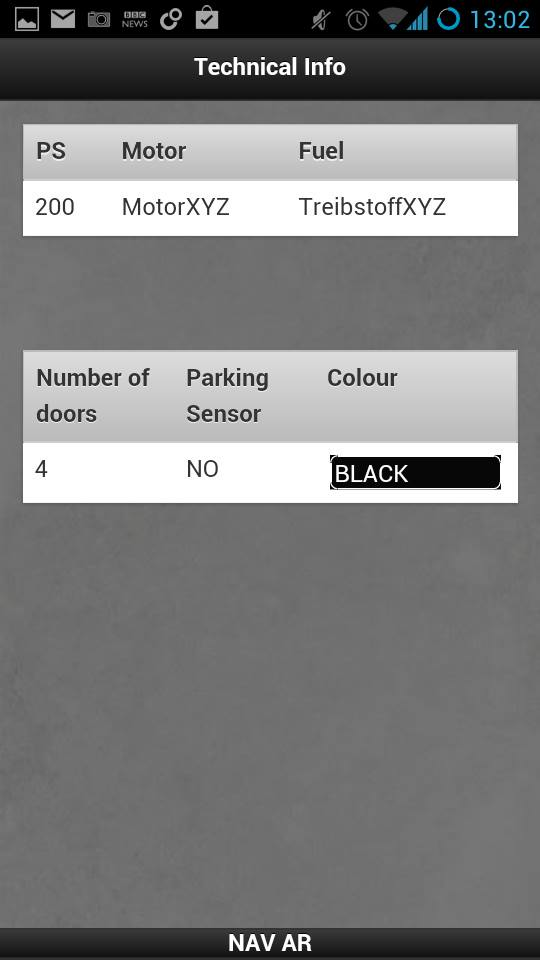
\includegraphics[width=0.4\linewidth]{graphics/chapter4/6.png}
\caption{Table}
\end{figure}
\clearpage
The second picture shows how the dynamic List of items from the Selector looks like:

\begin{figure}[h]
\centering
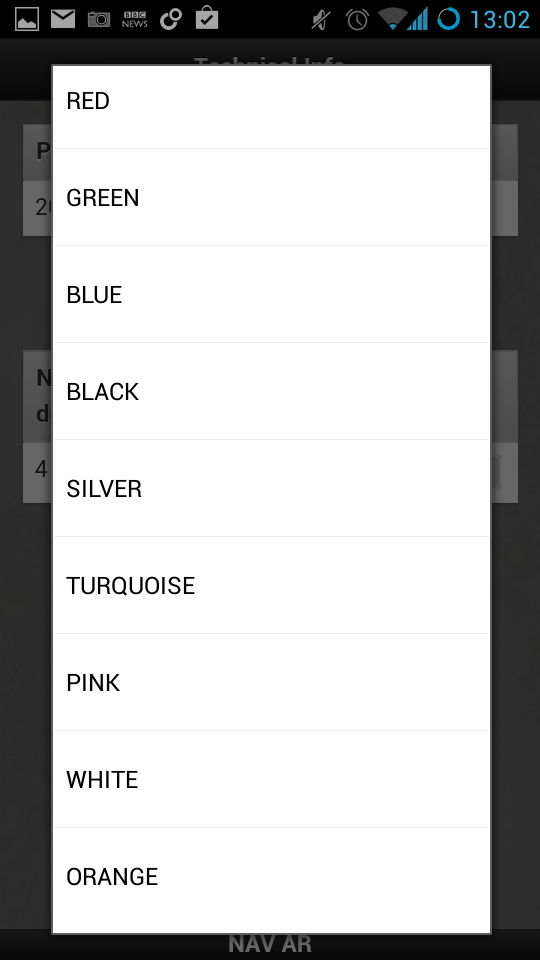
\includegraphics[width=0.4\linewidth]{graphics/chapter4/fg6.png}
\caption{Selector}
\end{figure}
\clearpage
Furthermore there is  a logic implemented which checks if the Colour is white or Black , that changes the colour of the font. The following code snippet shows how to write it:\\
\begin{figure}[h]
\centering
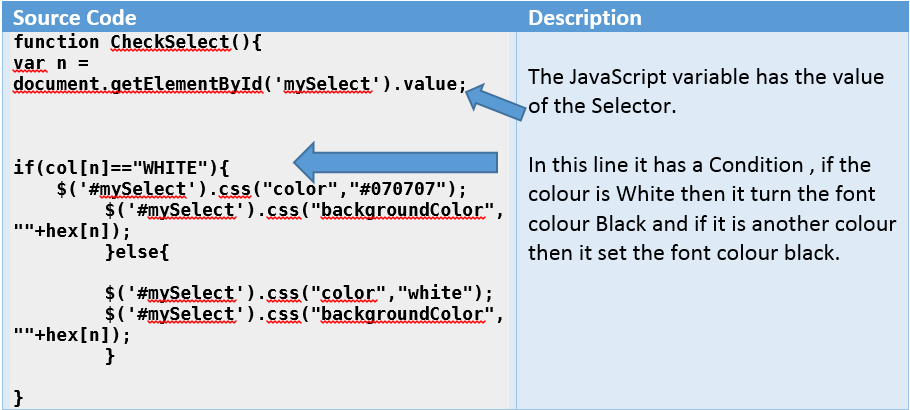
\includegraphics[width=1.0\linewidth]{graphics/bgfn.PNG}
\caption{Condition}
\end{figure}


% % % % % % % % % % % % % % % % % % % % % %

%%%%%%%%%%%%%%%%%%%%%%%%%%%%%%%%%%%%%%%%%
\chapter{Bibliographic Issues}
\label{ch:bibliographic}
%%%%%%%%%%%%%%%%%%%%%%%%%%%%%%%%%%%%%%%%%





\section{Literature Search}

Information on online libraries and literature search, e.g., interesting magazines, journals, conferences, and organizations may be found at \url{http://www.big.tuwien.ac.at/teaching/info.html}.

\section{BibTeX}

BibTeX should be used for referencing.

The LaTeX source document of this pdf document provides you with different samples for references to journals~\cite{jour:B2BServices}, conference papers~\cite{proc:TheWebMLApproach}, books~\cite{book:umlatwork}, book chapters~\cite{incoll:ErhardKonrad1992}, electronic standards~\cite{man:BPEL}, dissertations~\cite{phdthesis:manuelWimmer}, masters' theses~\cite{mast:AUMLProfile}, and web sites~\cite{misc:BIGWebsite}. The respective BibTeX entries may be found in the file \texttt{references.bib}. For administration of the BibTeX references we recommend \url{http://www.citeulike.org} or JabRef for offline administration, respectively.


%%%%%%%%%%%%%%%%%%%%%%%%%%%%%%%%%%%%%%%%%
%%% BACKMATTER %%%%%%%%%%%%%%%%%%%%%%%%%%
%%%%%%%%%%%%%%%%%%%%%%%%%%%%%%%%%%%%%%%%%

\appendix

\bibliographystyle{plain}
\bibliography{references}

\end{document}
